\chapter{PCB}
\label{cha:pcb}

\section{General Layout}

\fixme{This should be rewritten for my layout.}

The radar is constructed using a 4-layer board and uses both surfaces of the board. The front layer
contains nearly all of the board's components while the back layer contains a few surface mount
resistors and capacitors. The top layer primarily contains signal traces for top layer SMD
components. In particular, it connects many of the signal traces of the ADC to the FPGA, which is
placed next to it. Note, however, that most of the signal traces extending from the FPGA only start
on the top layer but travel through layer 3. The buck converters and subsequent linear regulators
are placed near the top of the board, not necessarily near the components they drive. In addition to
the large number of signal traces, the top copper layer contains a large ground plane around the
periphery of the board. The 2nd layer is entirely a ground plane. The 3rd layer is largely a ground
plane, although it also contains a significant number of traces extending from the FPGA as well as a
few other components. The 4th layer primarily contains large power planes for each of the different
voltages driving logic in the design. It is worth noting that even though it contains significant
power planes, it still has a ground plane that is the largest copper fill zone in this layer. The
PCB also has 3 large corner mounting vias with smaller vias placed in a circle in the large via's
annular ring. The reason for the small vias is to ensure a continued connection to GND (the mounting
vias are connected to GND) even if a screw thread strips too much copper from the main
via. Additionally, it helps prevent the PCB from being crushed if too much torque is used to tighten
the screw. The 4th corner is occupied by the connections to the DC barrel jack. Power rail traces
are made 0.5mm in width whereas signal traces are 0.2mm in width. Grounded vias are placed liberally
throughout the design. They have a diameter of 0.46mm and a drill hole size of 0.254mm. I've
included several screenshots of the PCB and highlighted important components
(Figures~\ref{fig:fmcw-layer1-layout}, ~\ref{fig:fmcw-layer1-gnd}, ~\ref{fig:fmcw-layer2-gnd},
~\ref{fig:fmcw-layer3-gnd}, ~\ref{fig:fmcw-layer4-gnd}, ~\ref{fig:fmcw-layer4-12v},
~\ref{fig:fmcw-layer4-3v6}, ~\ref{fig:fmcw-layer4-3v0}, ~\ref{fig:fmcw-layer4-3v3a},
~\ref{fig:fmcw-layer4-3v3d}, ~\ref{fig:fmcw-layer4-5v}, ~\ref{fig:fmcw-layer4-5vf}).

\begin{figure}[h]
        \centering
        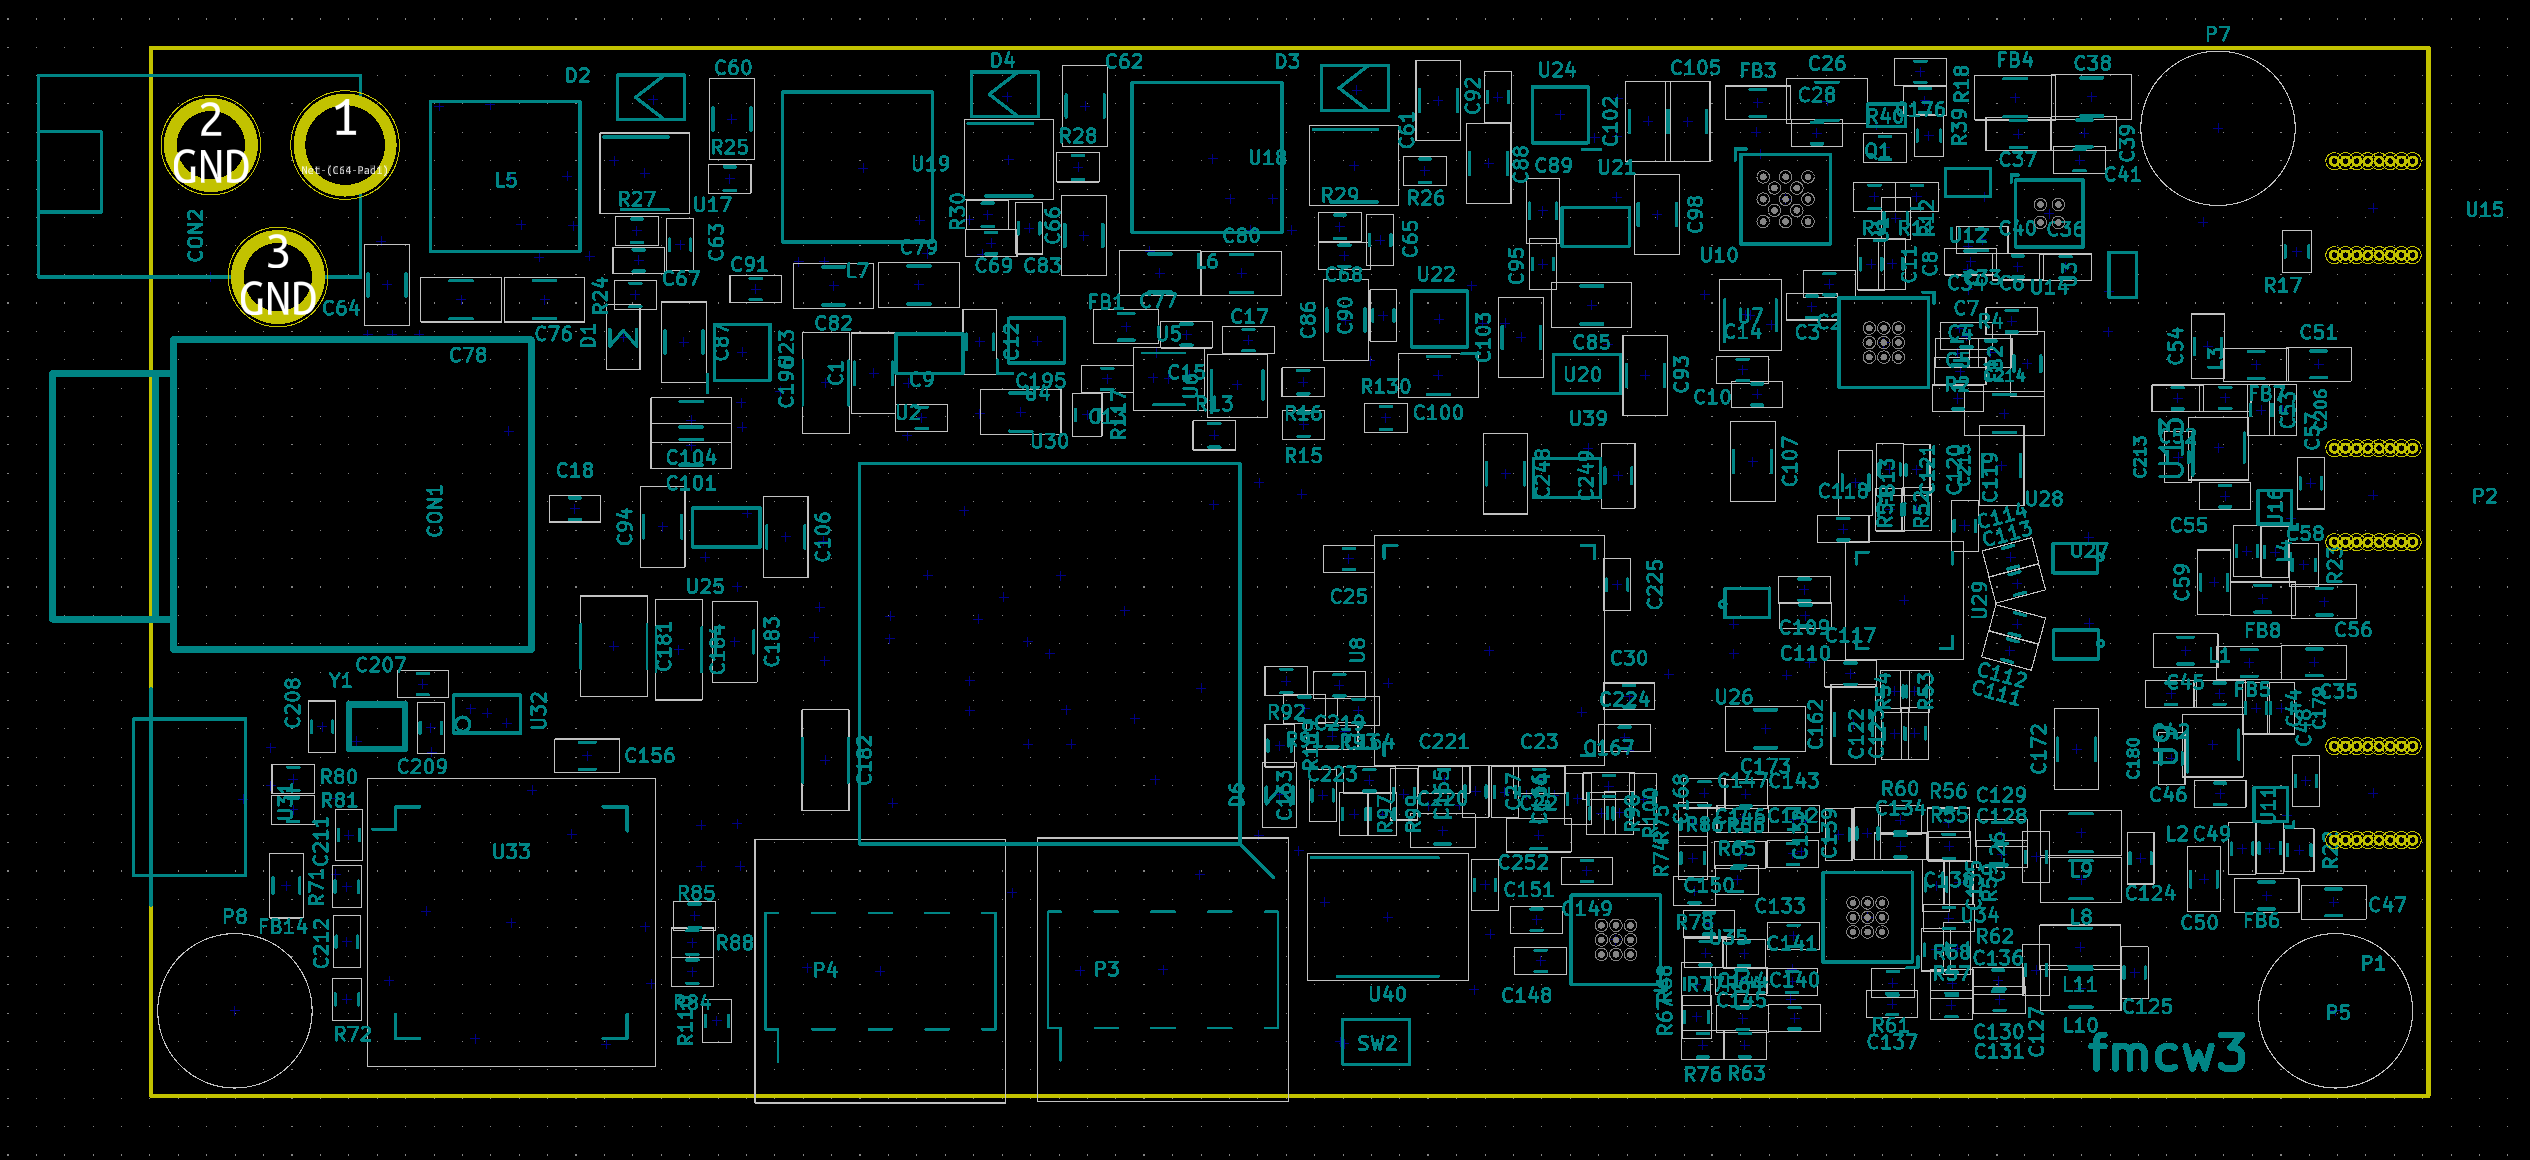
\includegraphics[width=\textwidth]{data/fmcw-layer1-layout.png}
        \caption{\textbf{Board layout}. The top left of the board is where the power source (barrel
          jack) is connected. The output of the 12V power source is connected to a power plane at
          the top left-middle of the board, that feeds into the buck converters. Large inductors
          connected to the buck converters are placed adjacent to their corresponding buck
          converters. The outputs of the buck converters feed into linear regulators that are mostly
          placed directly below the buck converters. This is also the region where the main crystal
          oscillator is placed and its associated fan-out buffer. Transmission circuitry (the
          frequency synthesizer and some RF amplifiers) are placed at the upper right side of the
          board near the antenna connectors which are placed on the right side of the
          board. Circuitry for signal reception are placed along the right side, adjacent to the
          antenna connectors. The mixer is placed slight inward from here, vertically centered but
          toward the right side of the board. Below this are intermediate frequency op-amps that
          feed the mixed signal into an ADC located just above it and to the left (U8). Located just
          to the left of the IF amplifiers and below the ADC is a flash memory IC (U40) which feeds
          data to the FPGA (U30), located just to the left of the ADC. Connectors below the FPGA (P3
          and P4) can be used to externally monitor the FPGA. In the bottom left of the board is a
          component to convert USB data to UART data to configure the FPGA as well as a micro USB
          connection to connect to a host computer. On the left side of the board between the USB
          connection and barrel jack is a SD card reader that stores data that can be read back out
          the FPGA.}
        \label{fig:fmcw-layer1-layout}
\end{figure}

\begin{figure}[h]
        \centering
        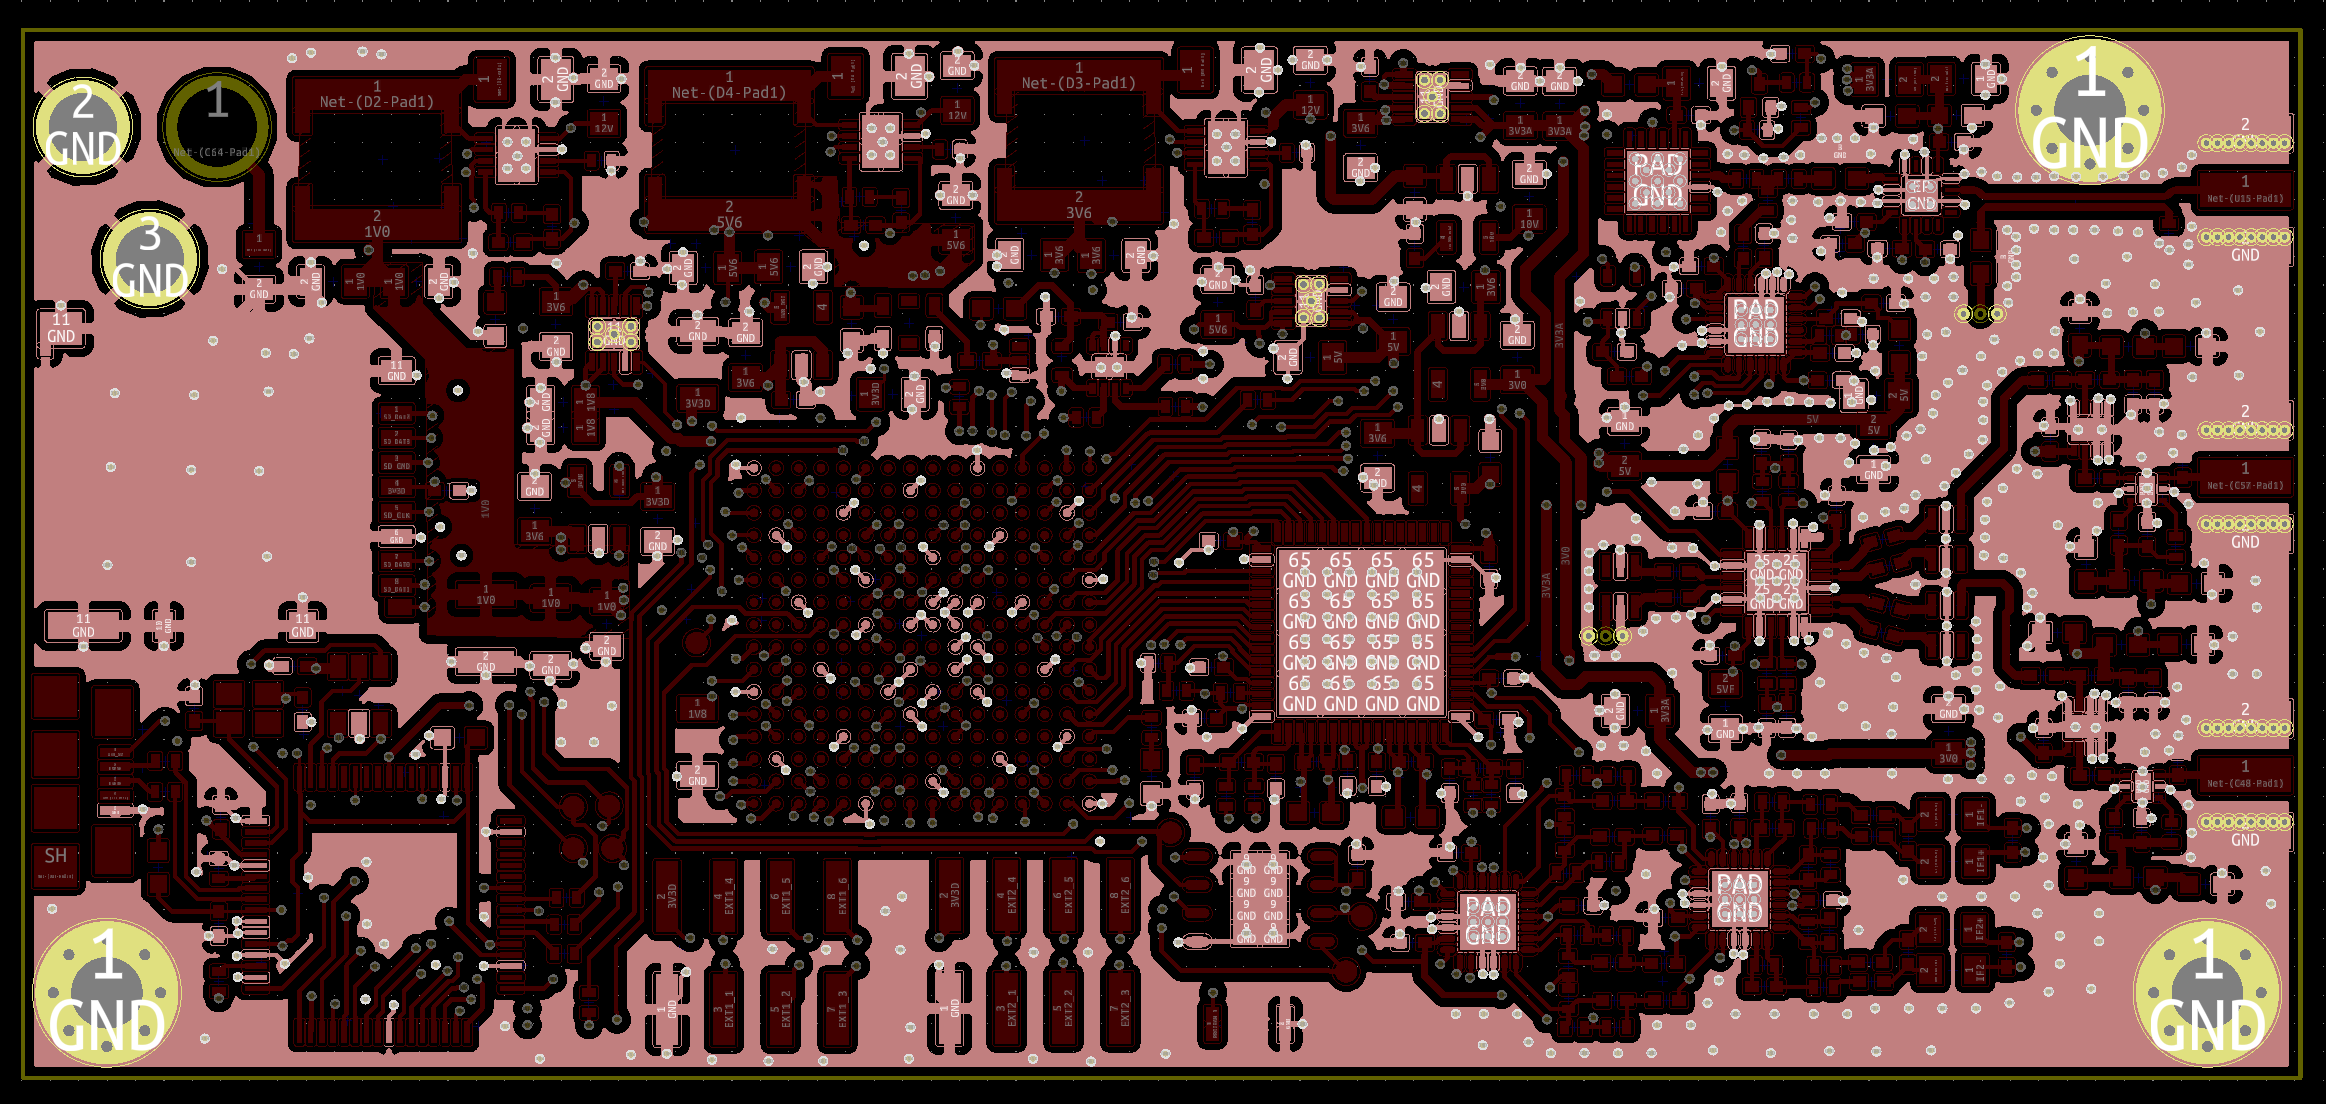
\includegraphics[width=\textwidth]{data/fmcw-layer1-gnd.png}
        \caption{A significant portion of layer 1 is a ground plane and the other large part of it
          is signal traces connecting components. There is also a small 1V power plane toward the
          upper left not highlighted here.}
        \label{fig:fmcw-layer1-gnd}
\end{figure}

\begin{figure}[h]
        \centering
        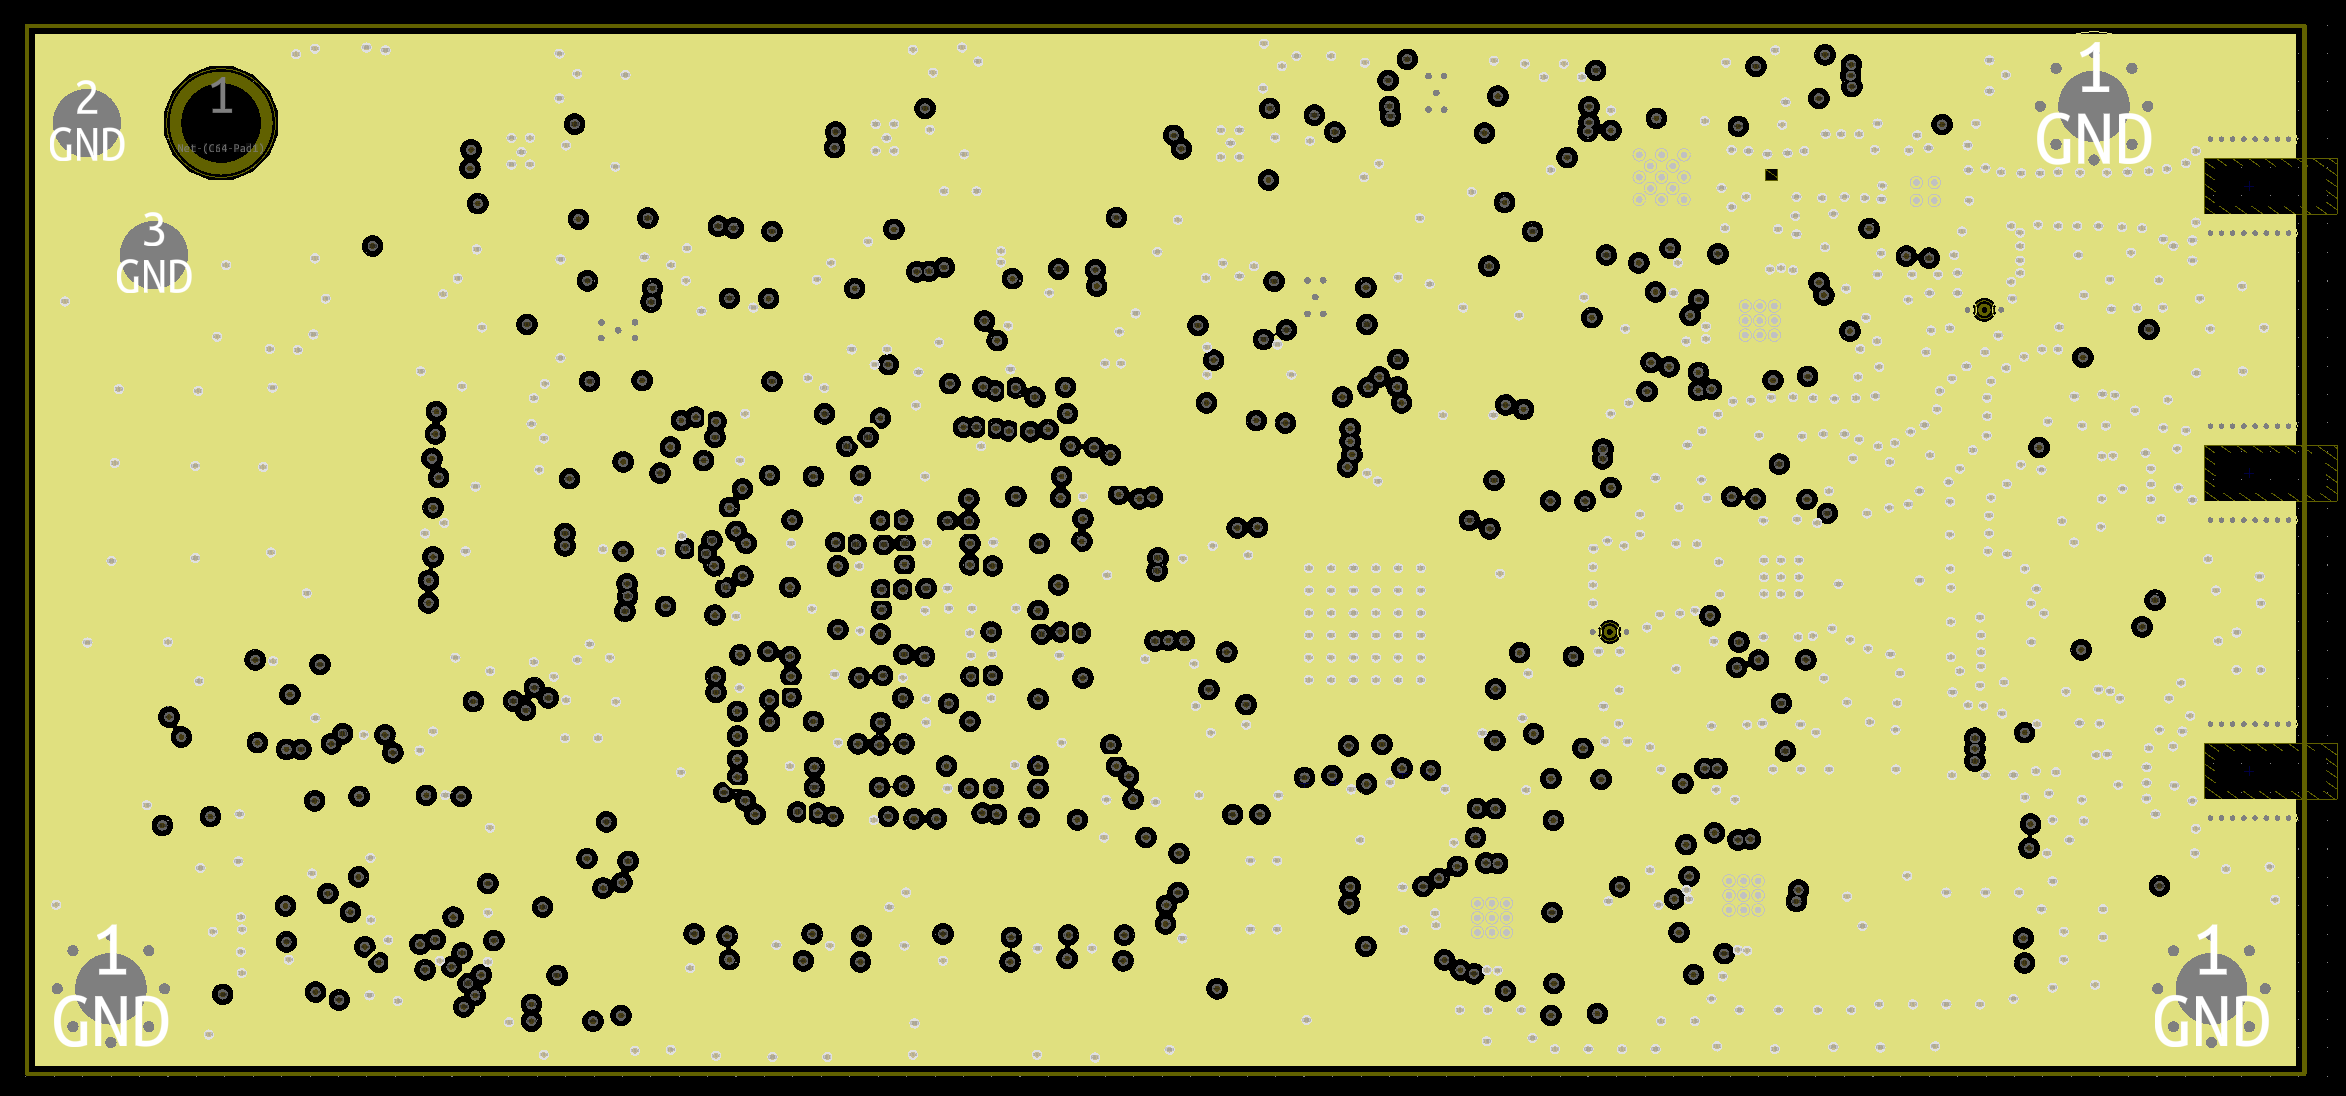
\includegraphics[width=\textwidth]{data/fmcw-layer2-gnd.png}
        \caption{All of layer 2 is a ground plane.}
        \label{fig:fmcw-layer2-gnd}
\end{figure}

\begin{figure}[h]
        \centering
        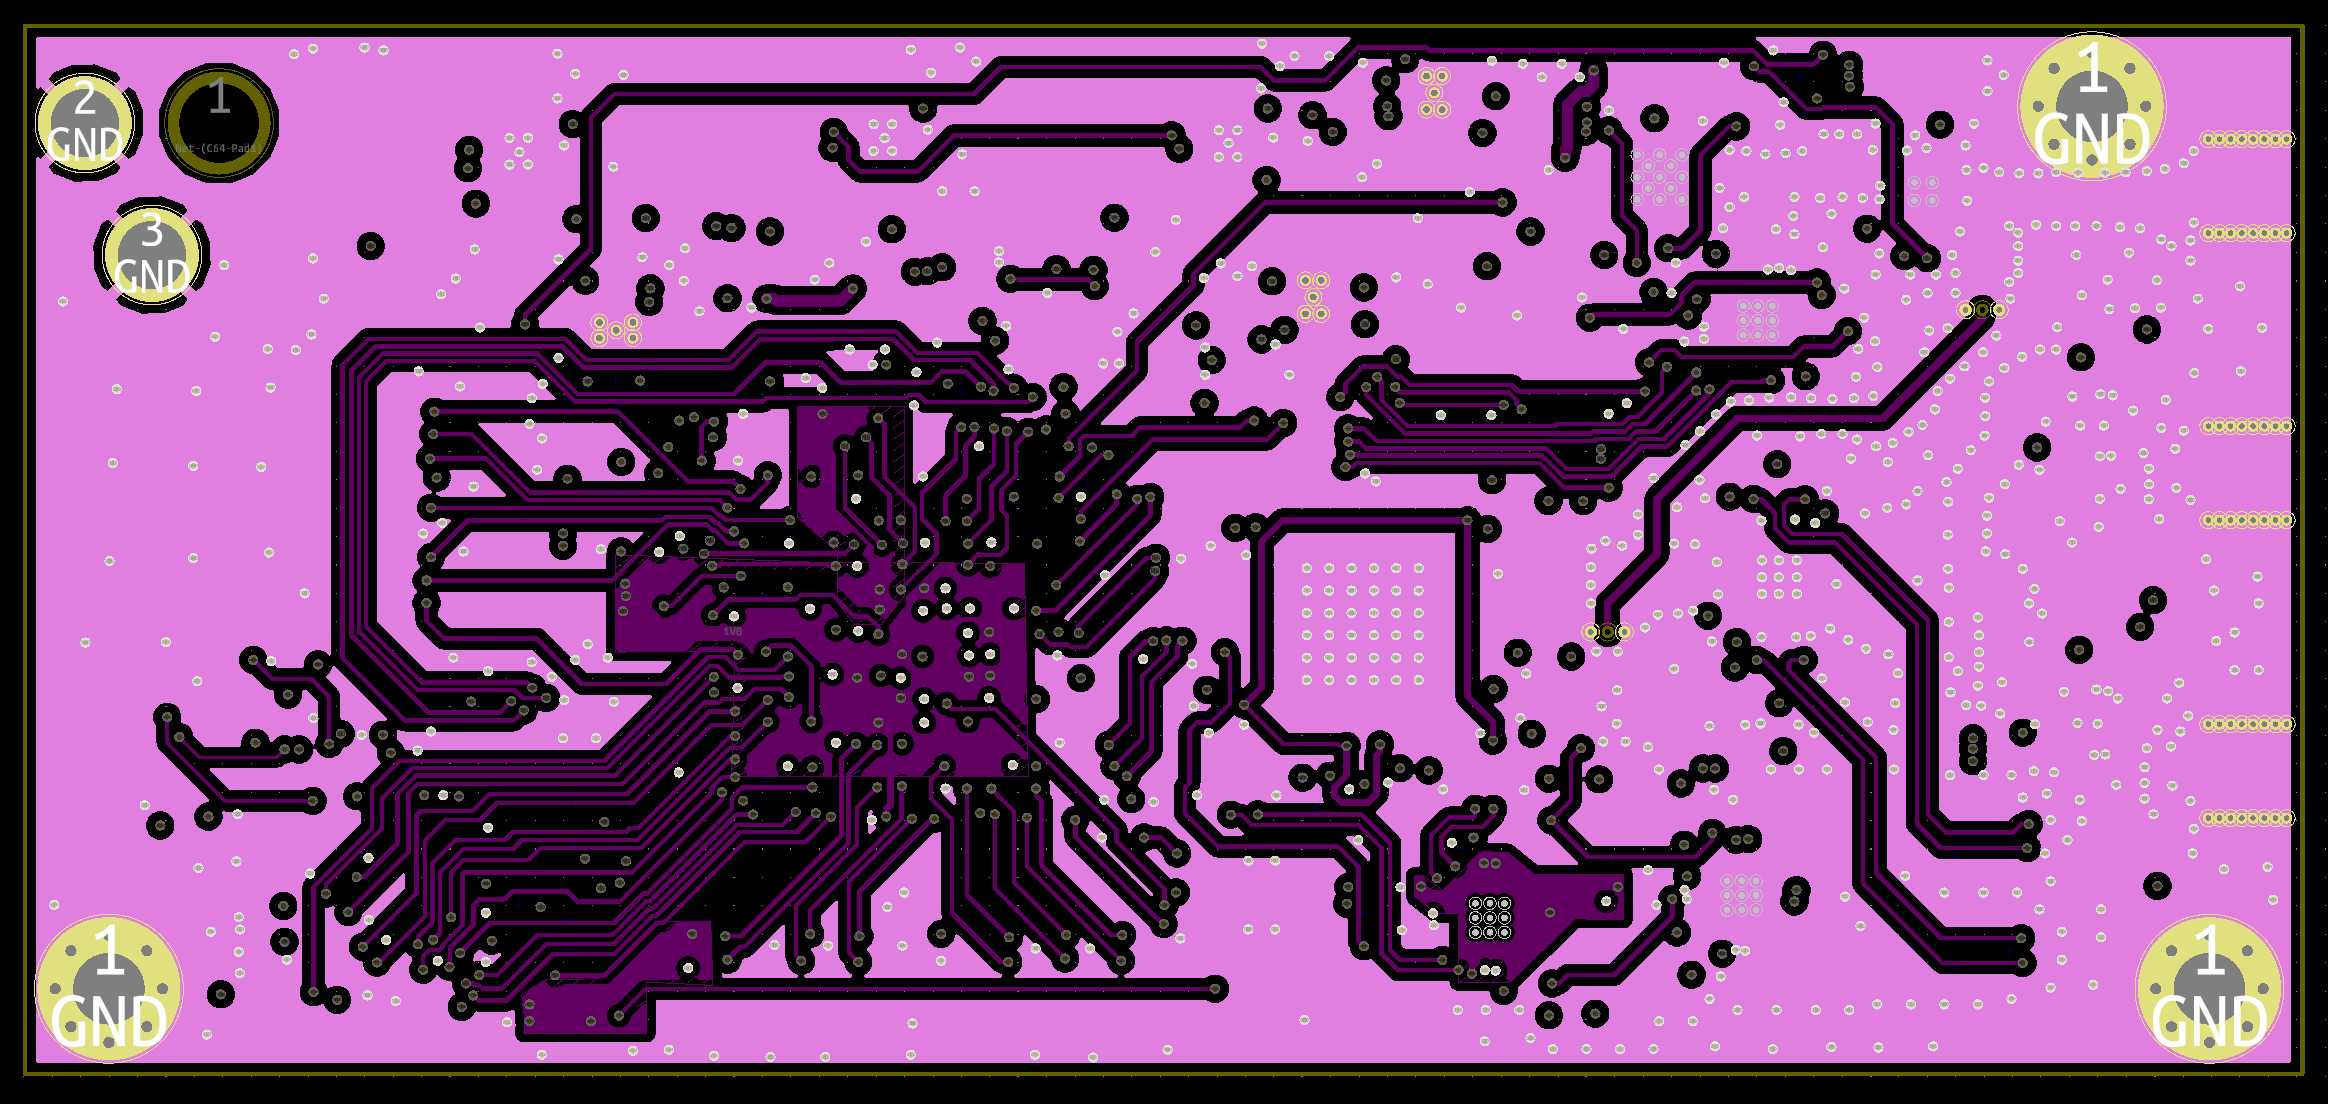
\includegraphics[width=\textwidth]{data/fmcw-layer3-gnd.png}
        \caption{Most of layer 3 is a ground plane but there are also a substantial number of trace
          connecting to the FPGA. It does also contain 1V an 3.3V power planes.}
        \label{fig:fmcw-layer3-gnd}
\end{figure}

\begin{figure}[h]
        \centering
        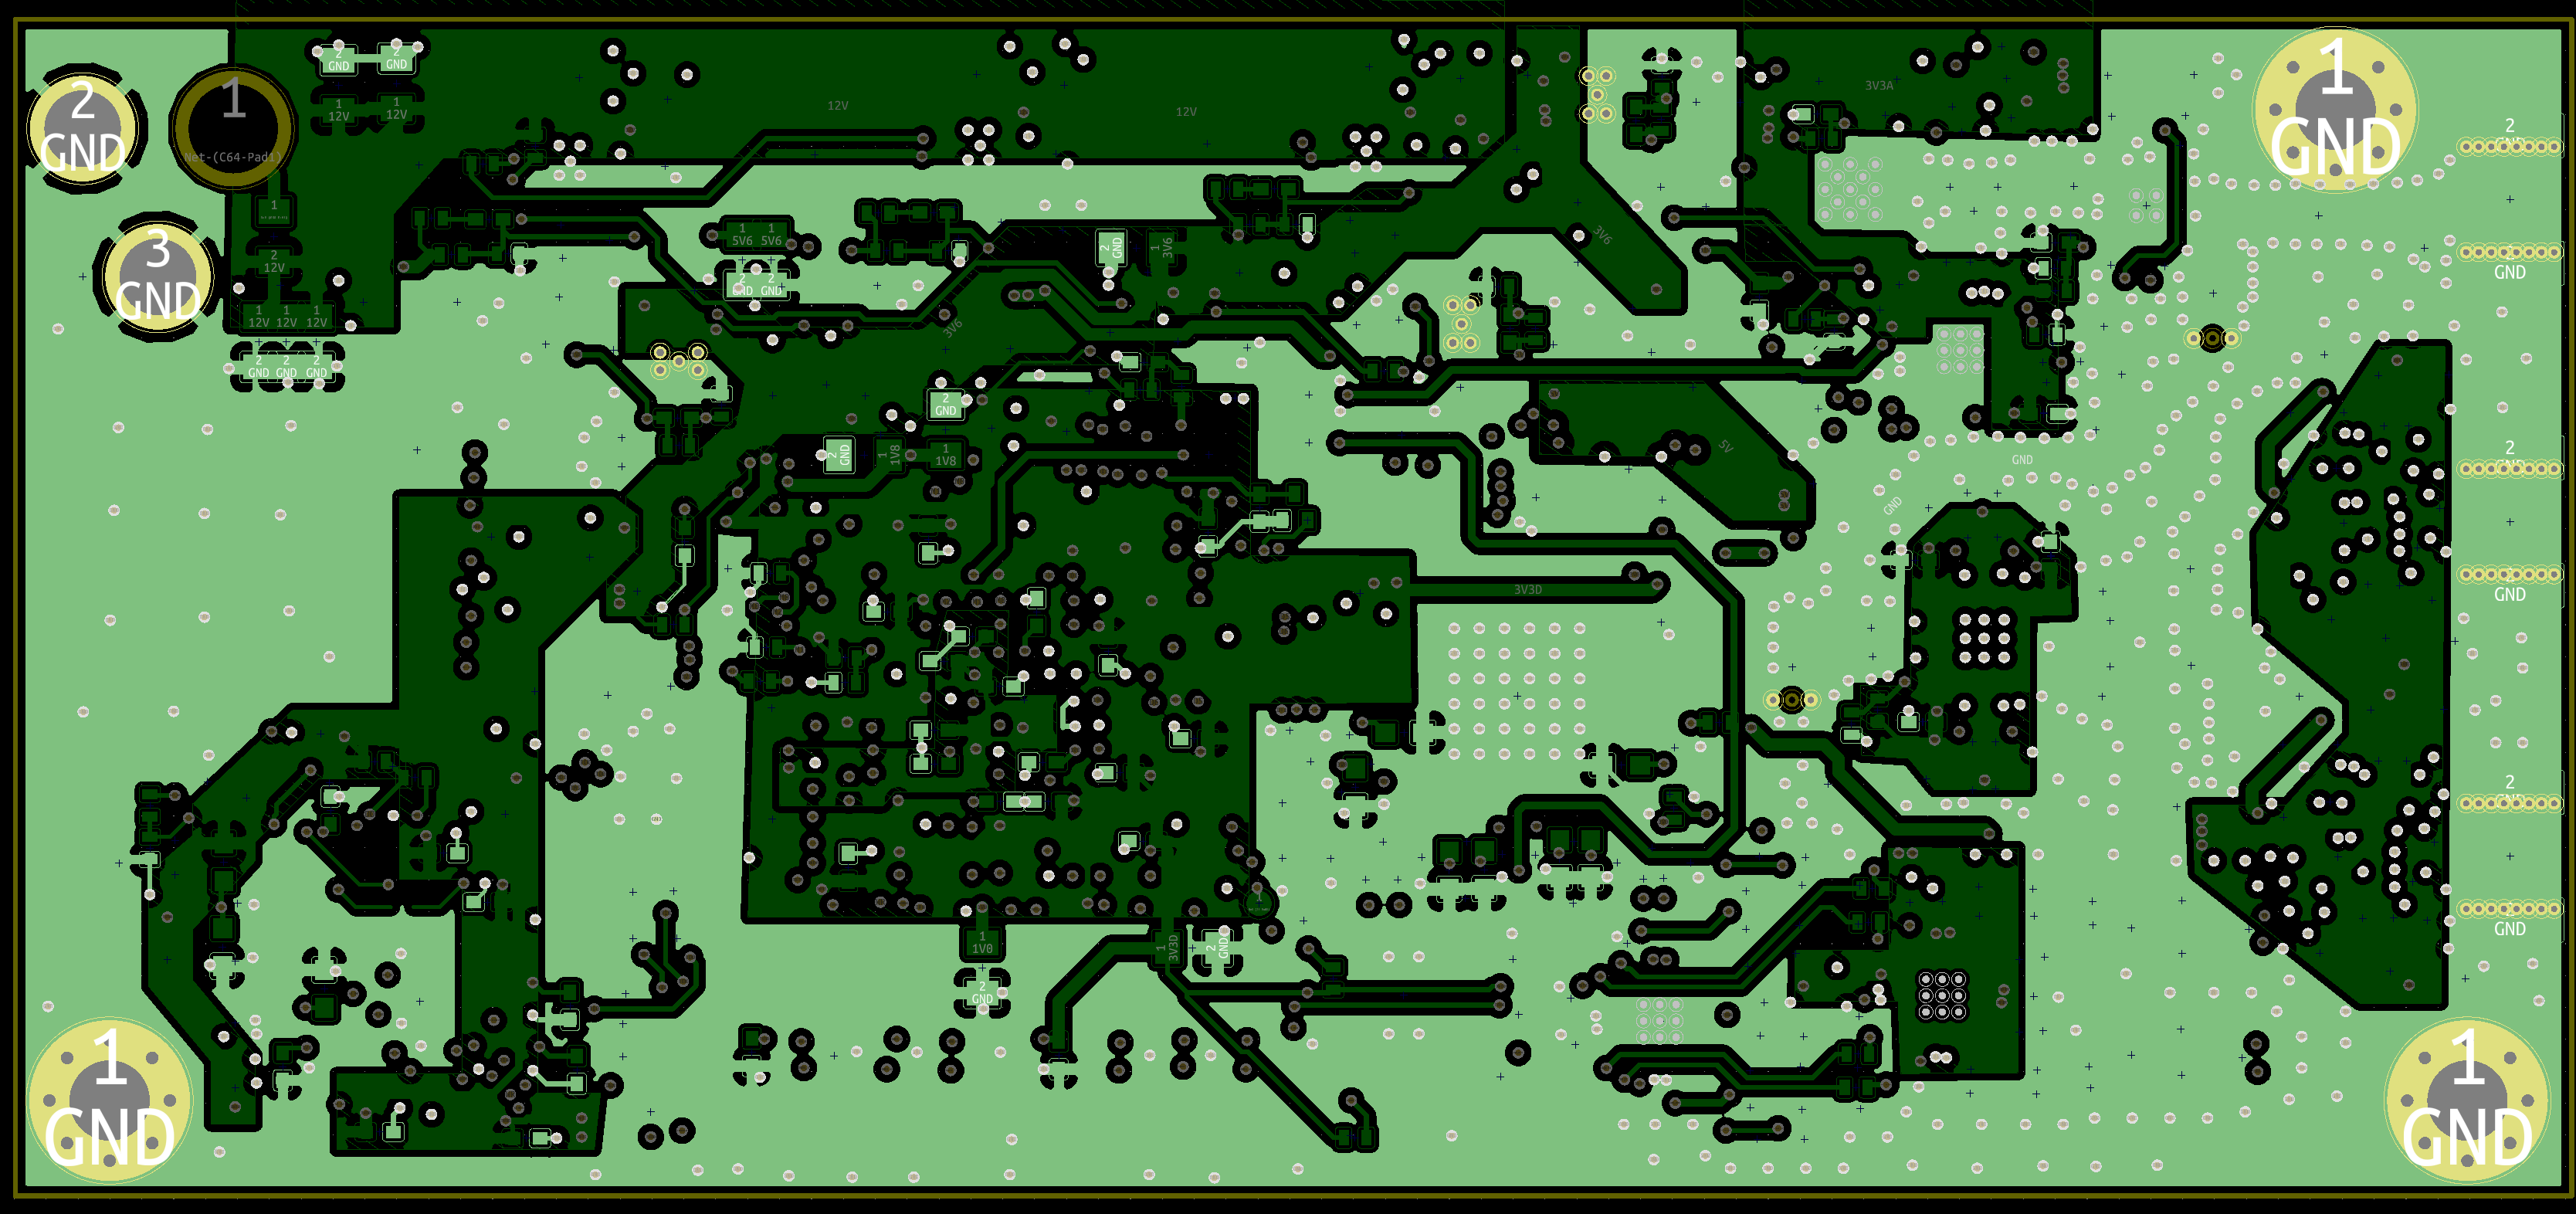
\includegraphics[width=\textwidth]{data/fmcw-layer4-gnd.png}
        \caption{The 4th layer of the PCB contains a large ground plane with many vias
          interspersed.}
        \label{fig:fmcw-layer4-gnd}
\end{figure}

\begin{figure}[h]
        \centering
        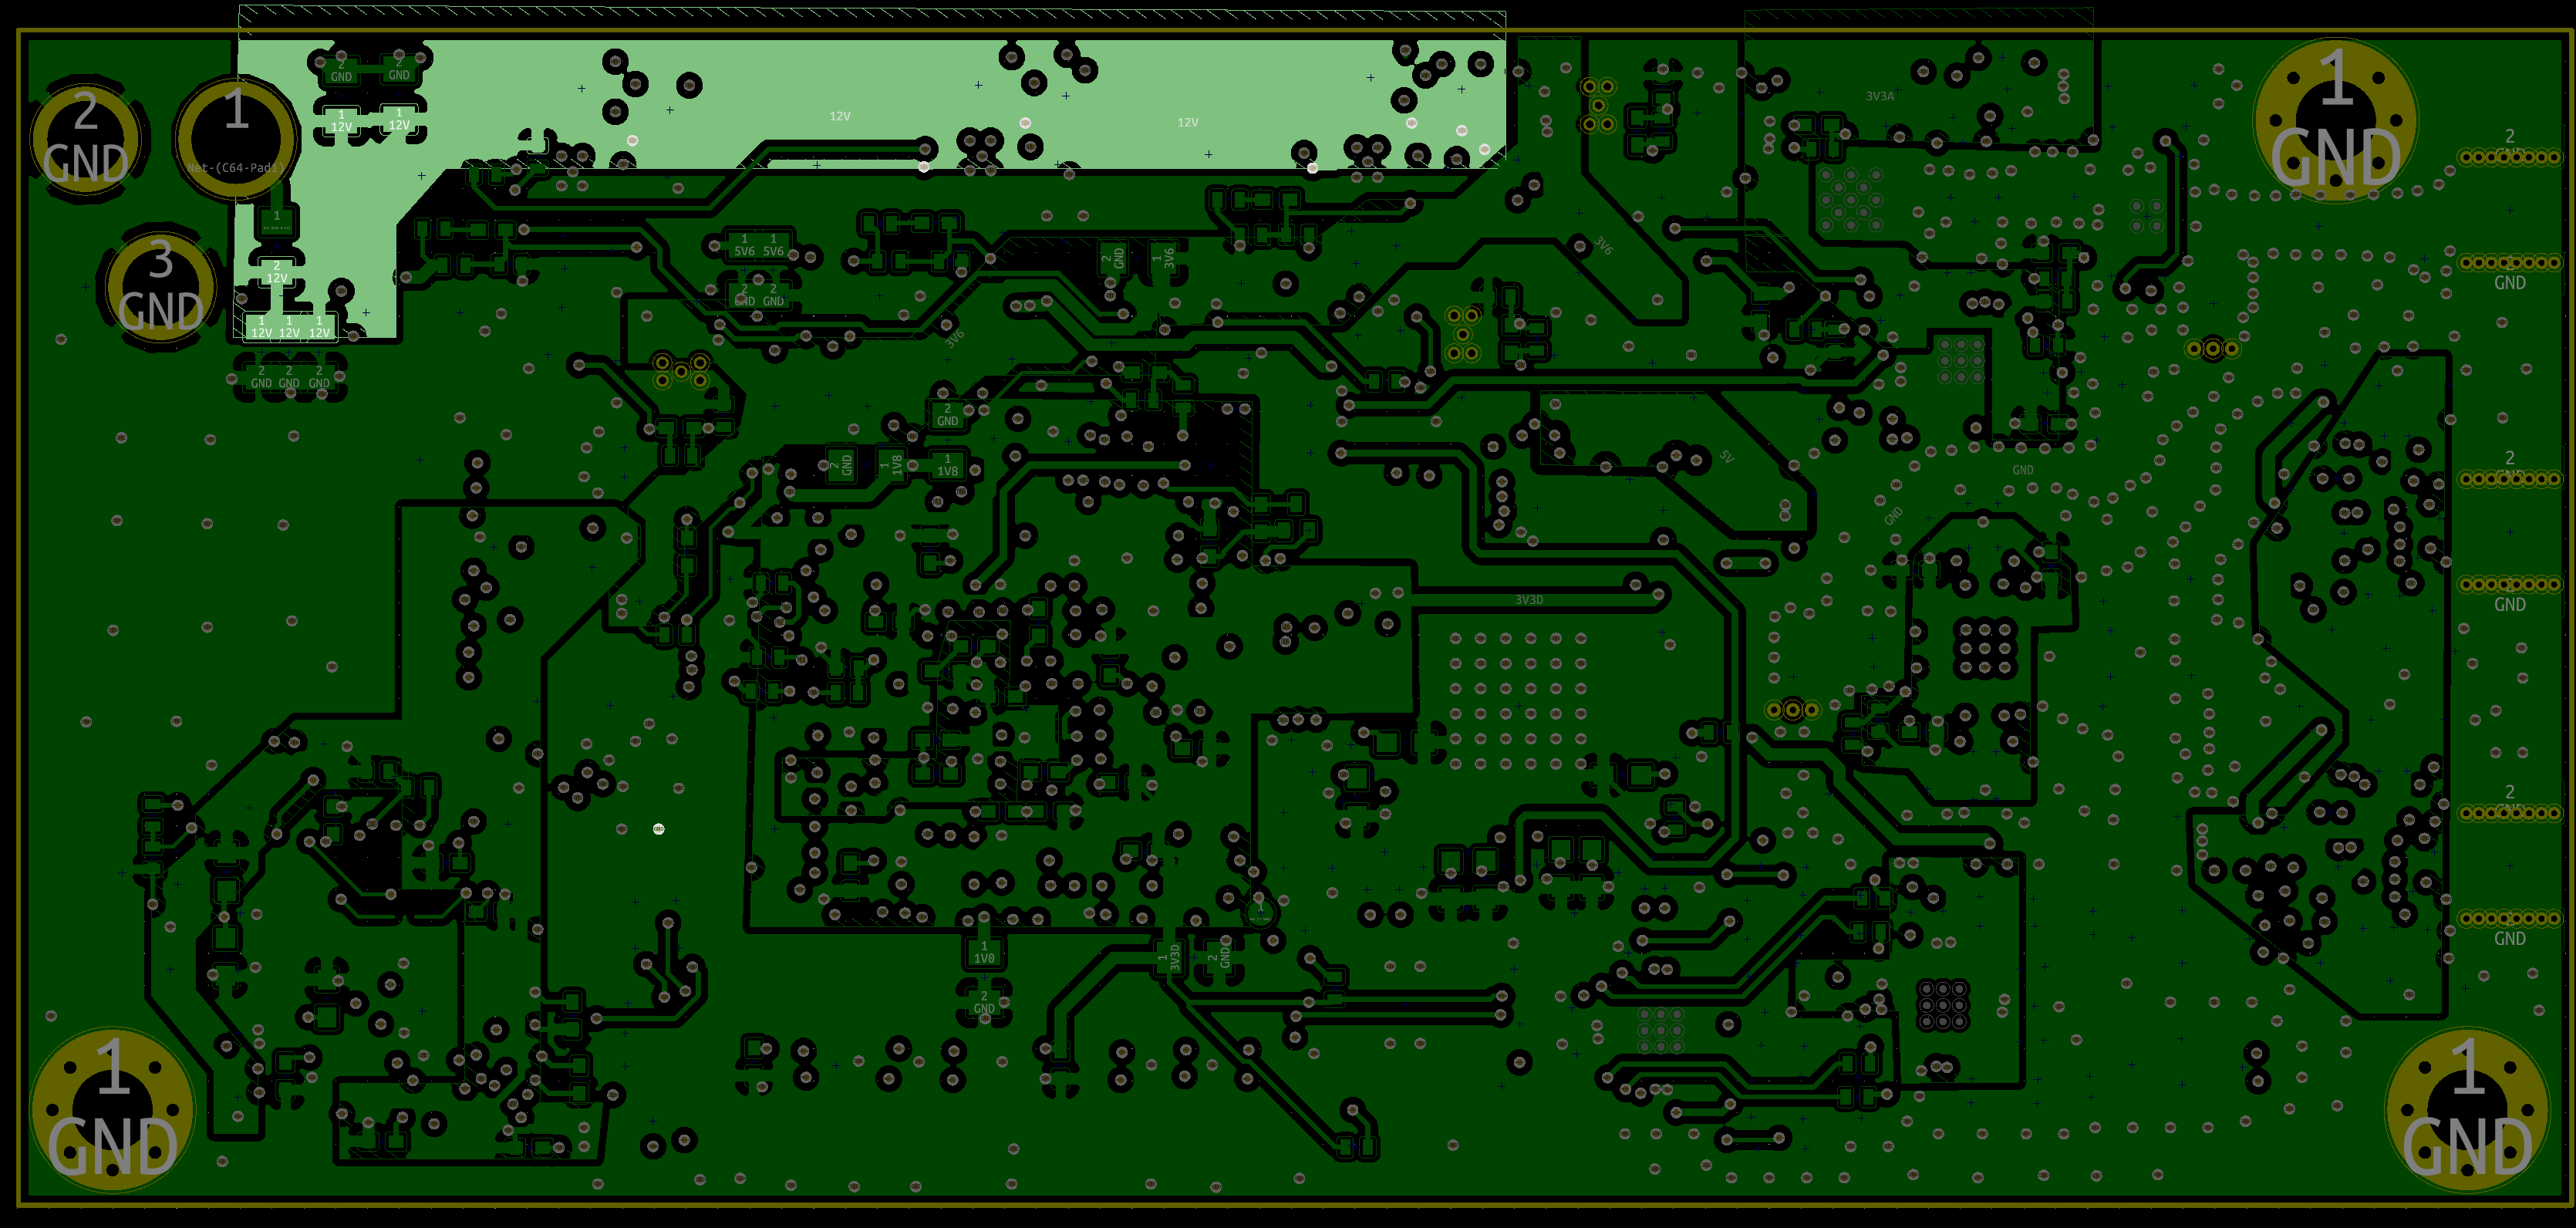
\includegraphics[width=\textwidth]{data/fmcw-layer4-12v.png}
        \caption{The 12V power plane is located at the top of the board adjacent to the D barrel
          jack and the buck converters it feeds.}
        \label{fig:fmcw-layer4-12v}
\end{figure}

\begin{figure}[h]
        \centering
        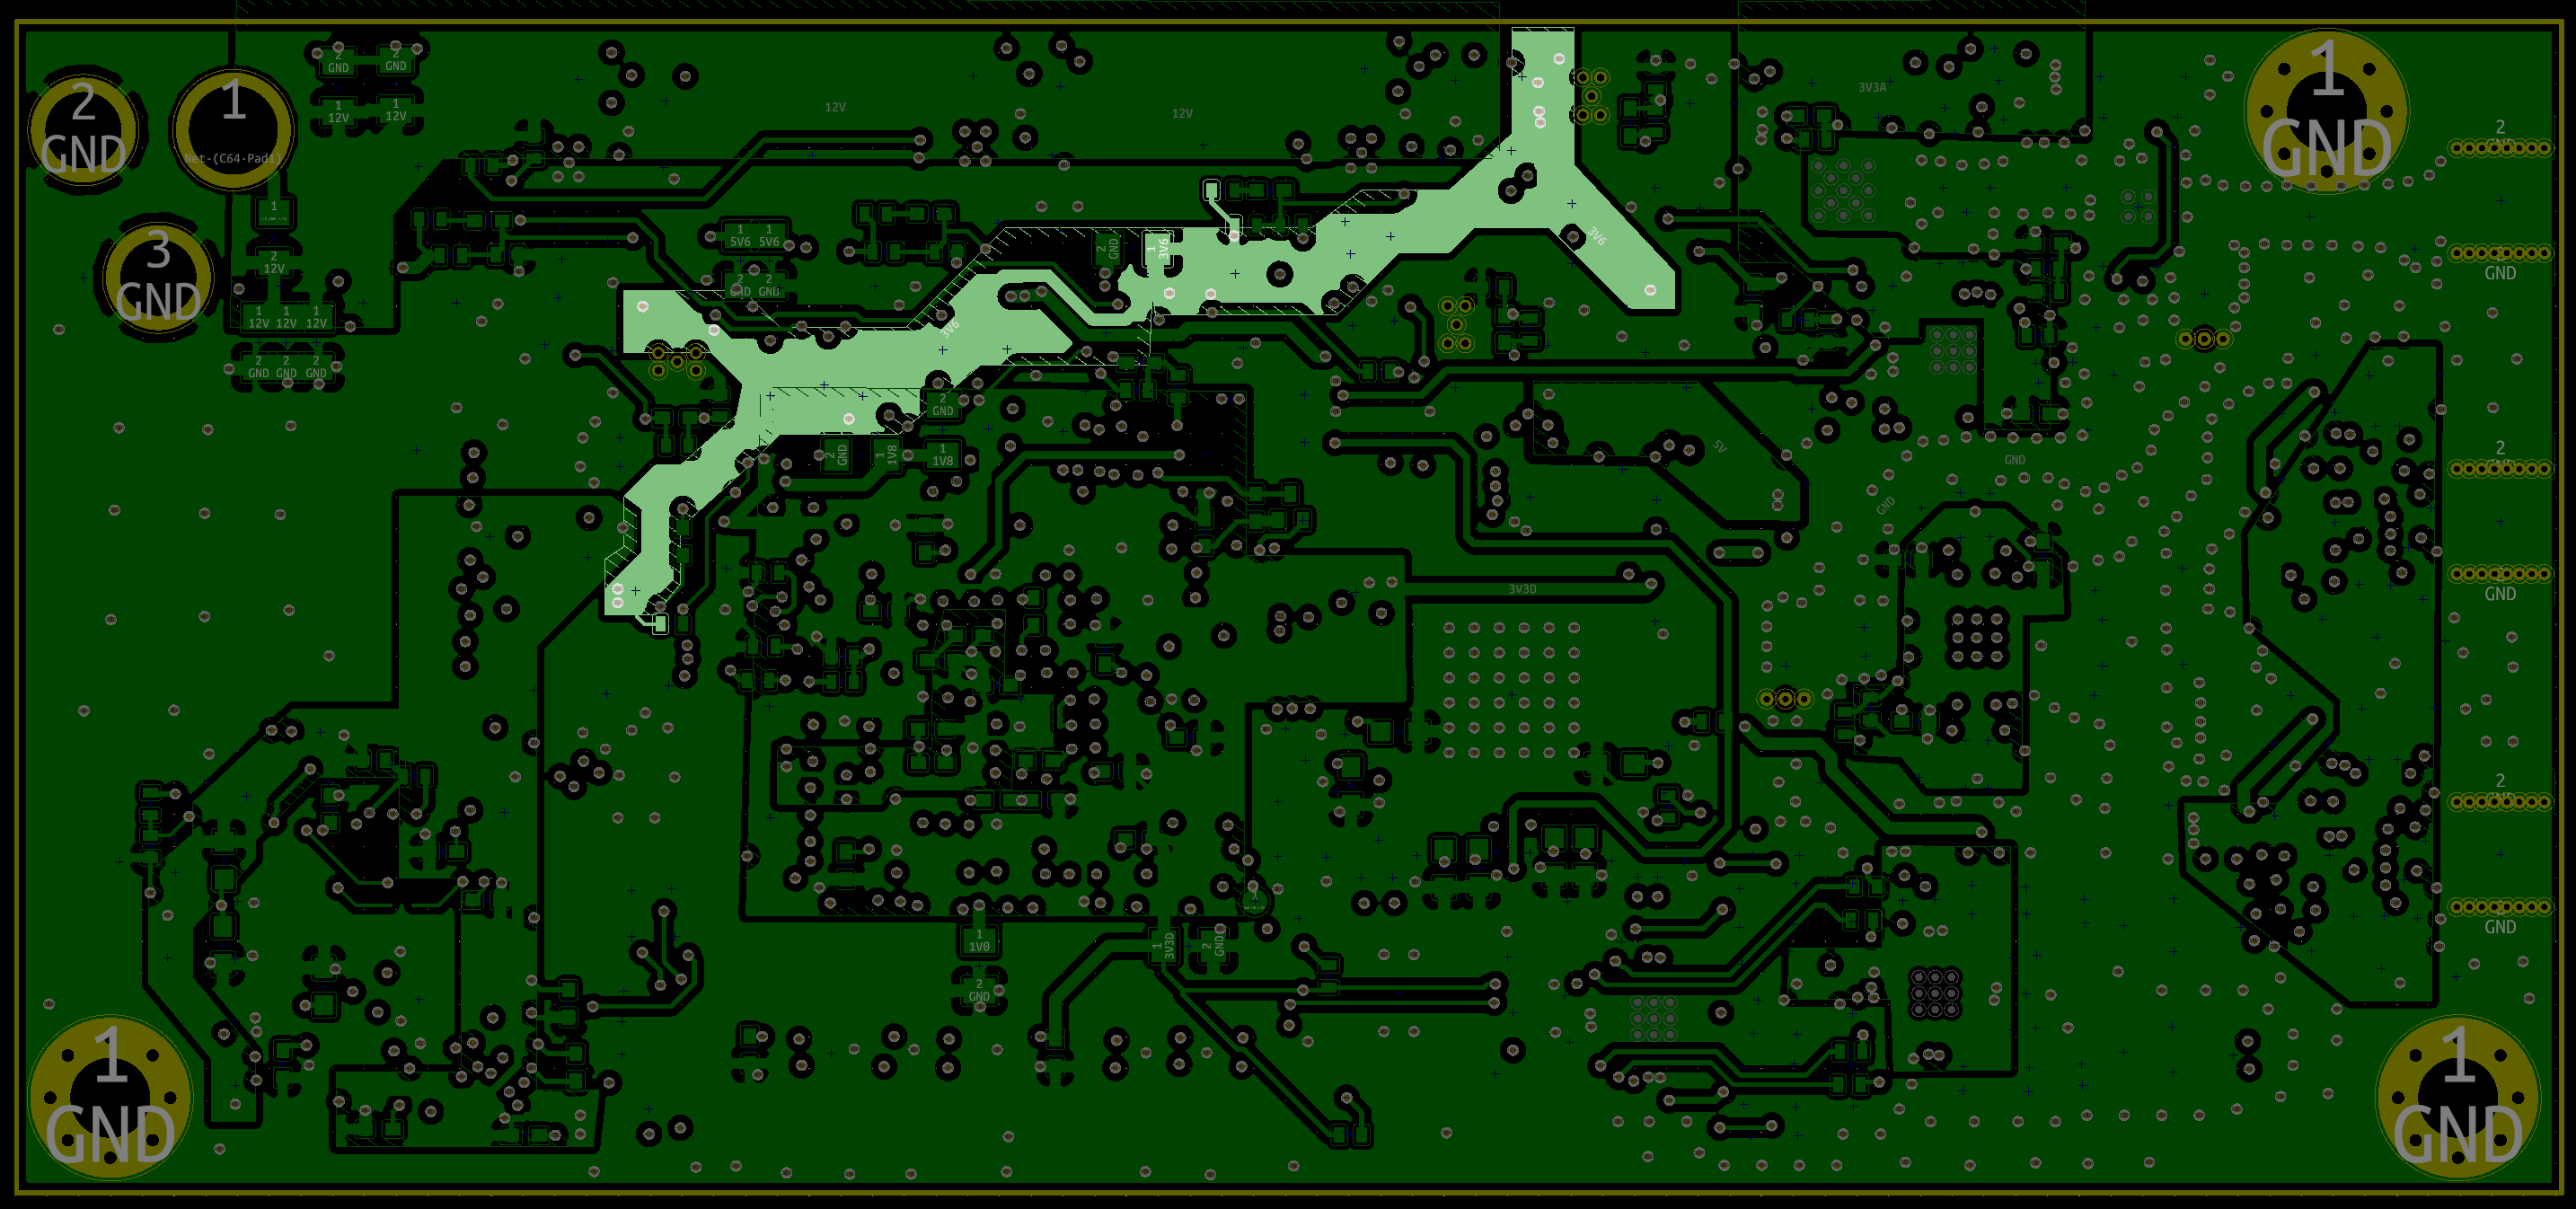
\includegraphics[width=\textwidth]{data/fmcw-layer4-3v6.png}
        \caption{There is a 3.6V power plane that is the output of one of the buck converter and is
          use as the input to several linear regulators that output 1.8V 3.0V and 3.3V.}
        \label{fig:fmcw-layer4-3v6}
\end{figure}

\begin{figure}[h]
        \centering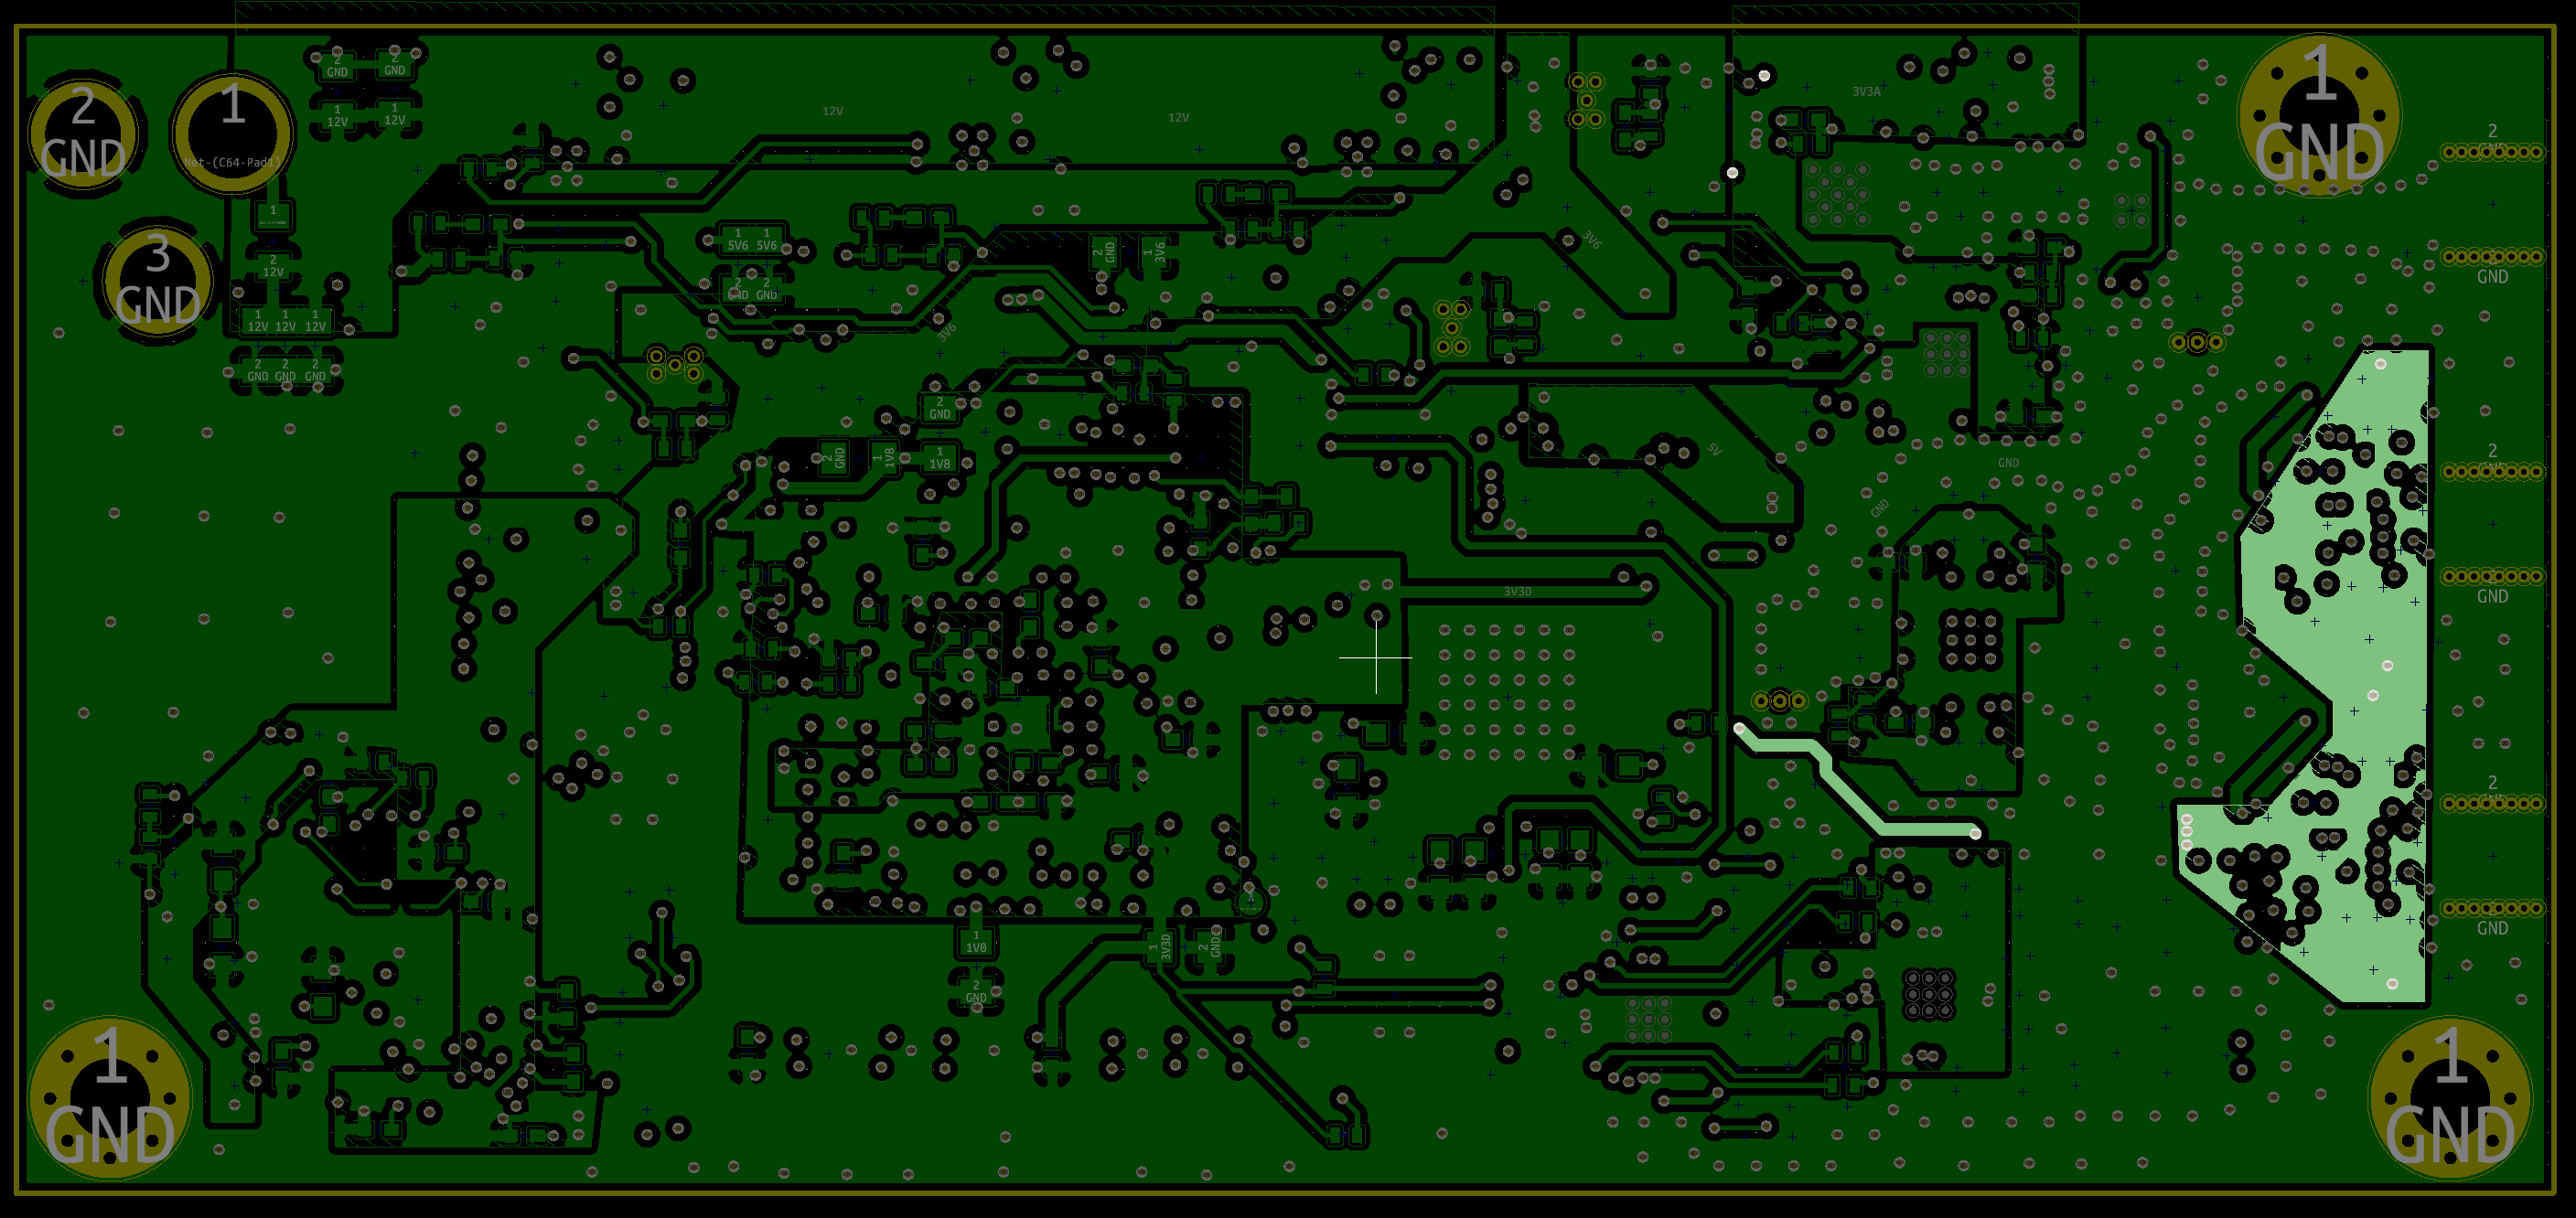
\includegraphics[width=\textwidth]{data/fmcw-layer4-3v0.png}
        \caption{A 3V power plane is used to power components near the right side of the boar (the
          righside of the board is where signal transmission and reception occur that amplify
          receive signals so they can be mixed with the transmitted signal and fed into the ADC
          before FPGA processing Notably, the 3V power plane is located near the components but far
          from the linear regulator that outputs it.}
        \label{fig:fmcw-layer4-3v0}
\end{figure}

\begin{figure}[h]
        \centering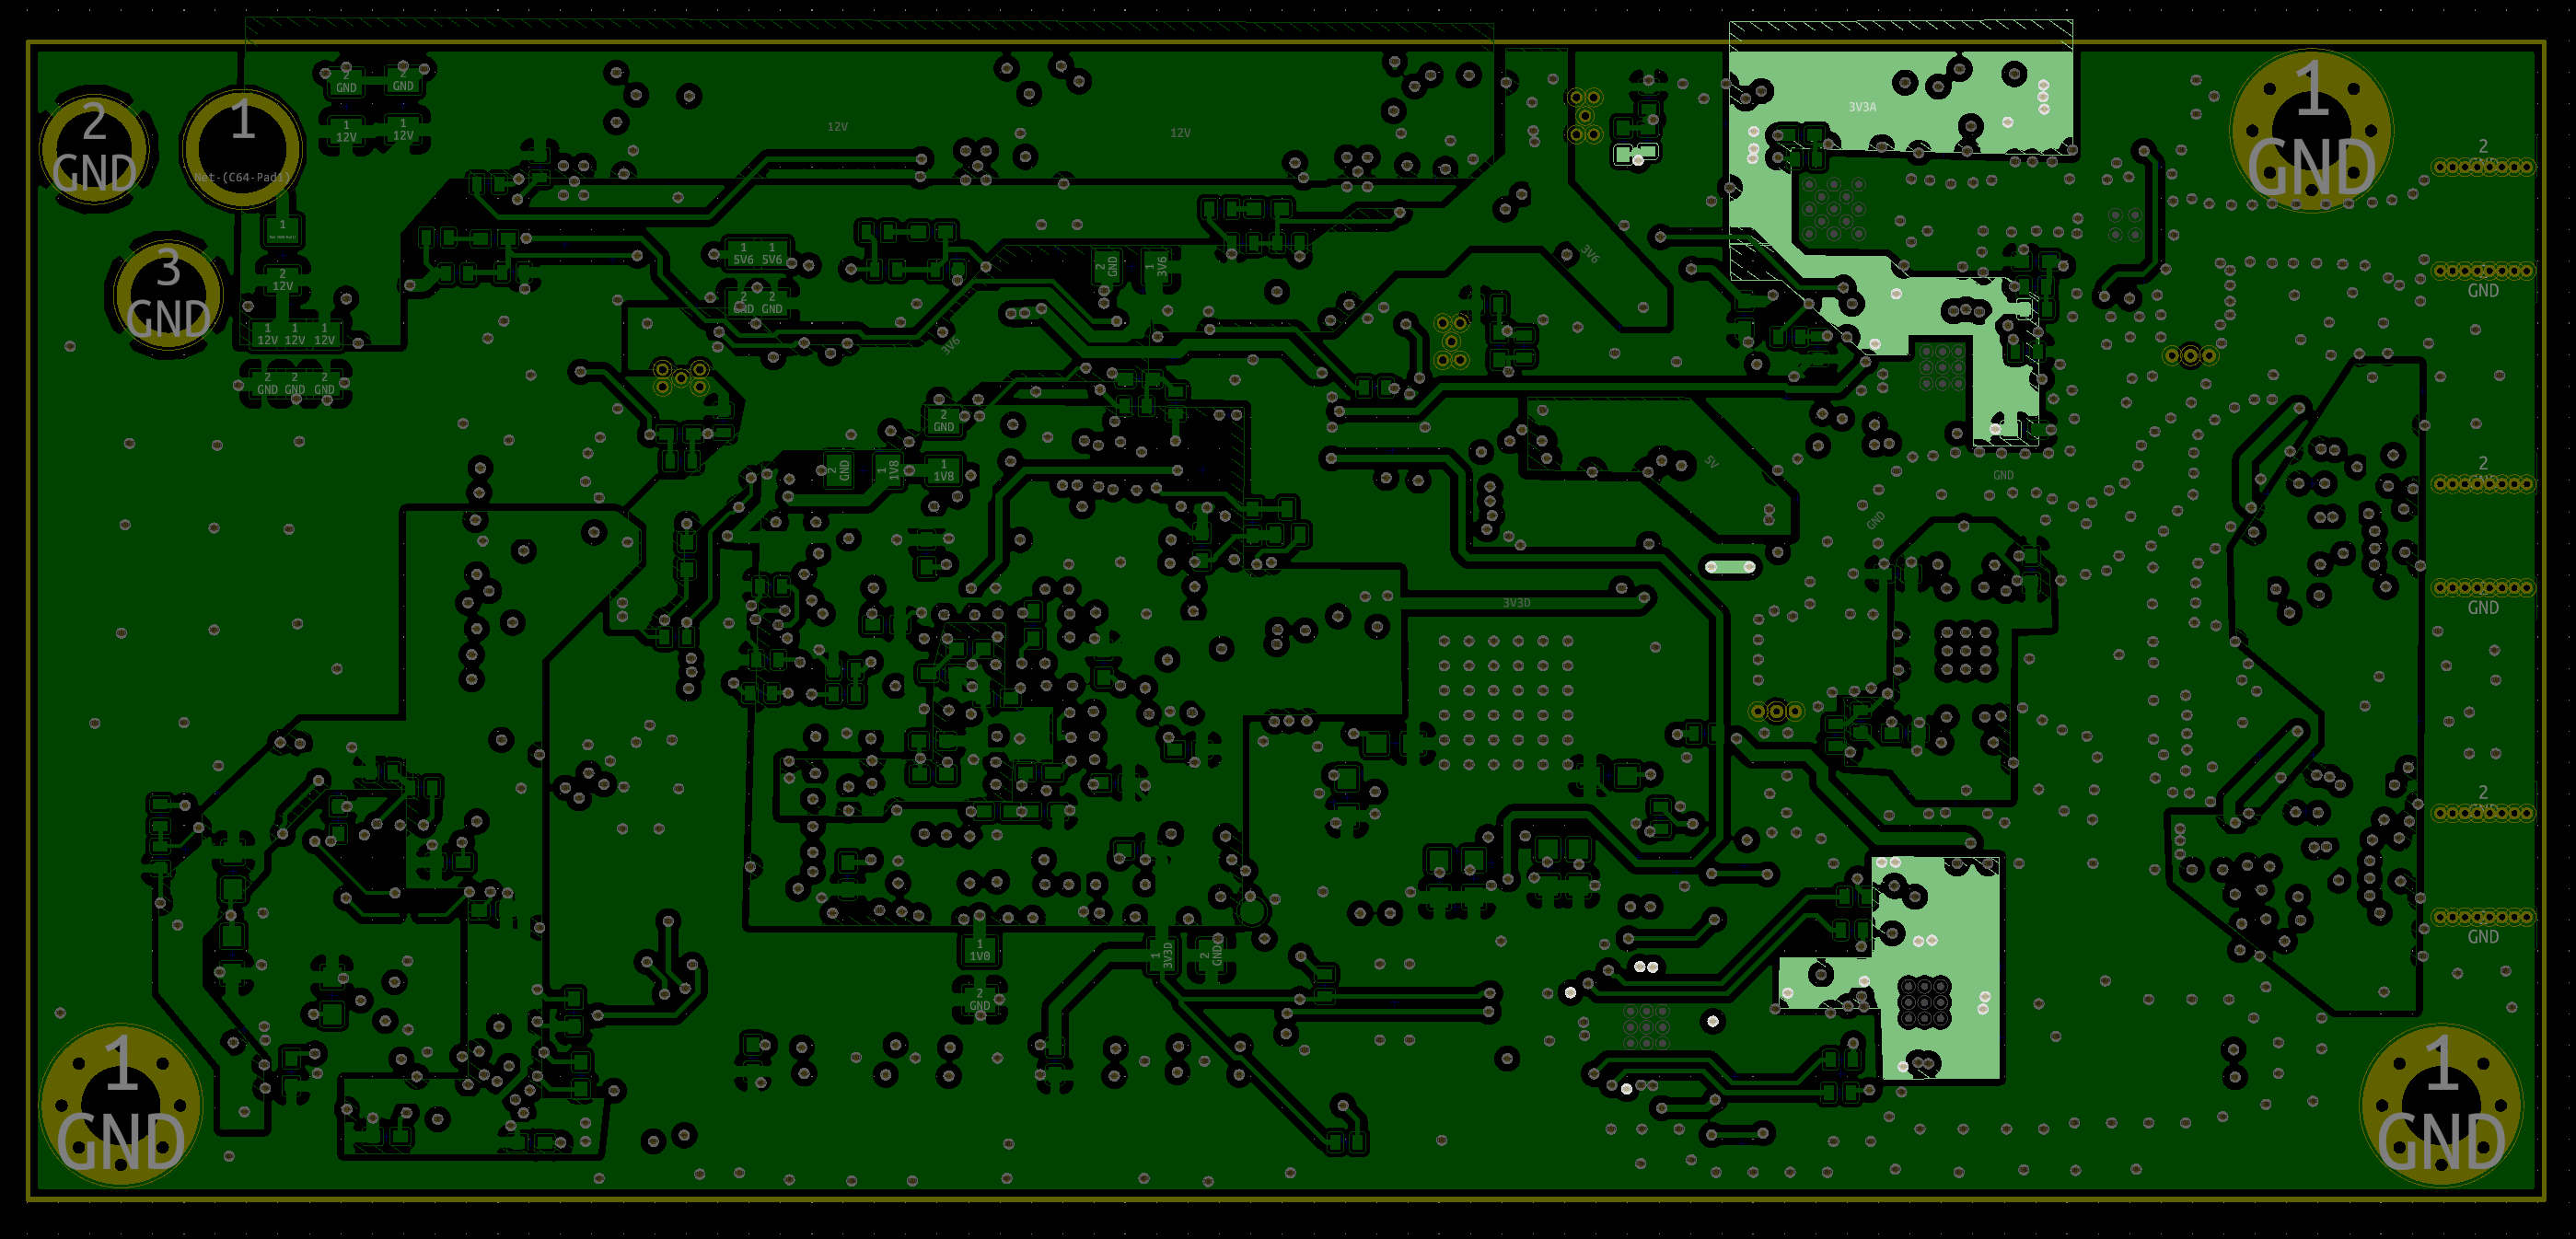
\includegraphics[width=\textwidth ]{data/fmcw-layer4-3v3a.png}
        \caption{A 3.3V power plane is used to power several components for signal transmission,
          such as a frequency synthesizer, and RF amplifier. These, along with all other reception
          and transmission circuitry, are located on the right side of the board.}
        \label{fig:fmcw-layer4-3v3a}
\end{figure}

\begin{figure}[h]
        \centering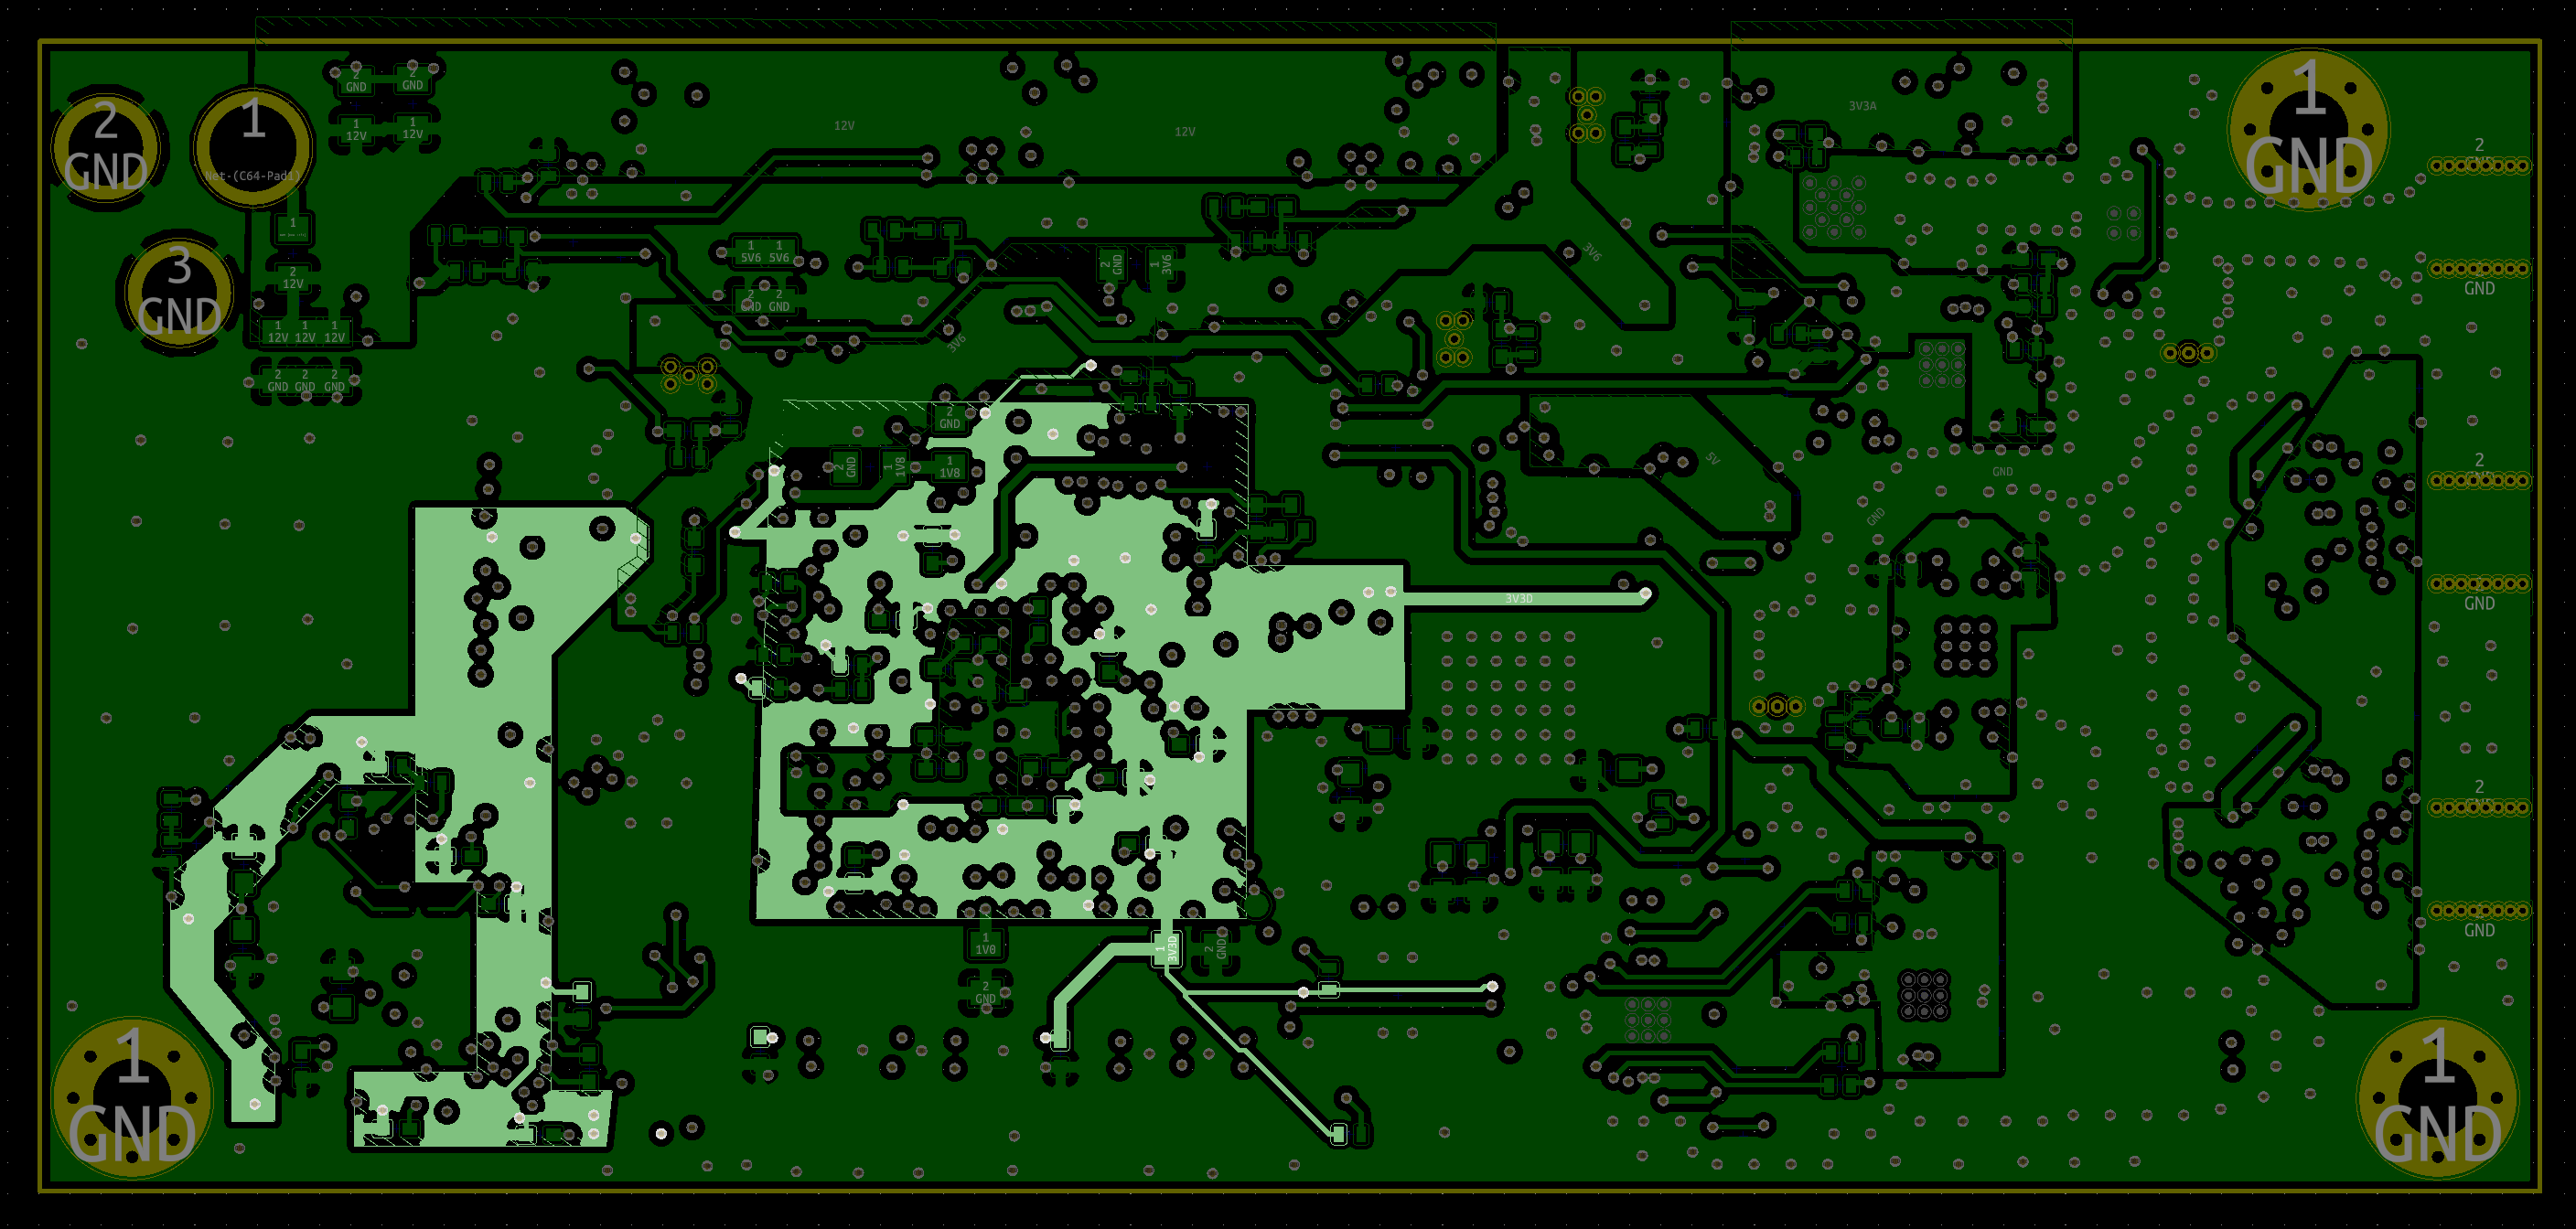
\includegraphics[width=\textwidth]{data/fmcw-layer4-3v3d.png}
        \caption{Another 3.3V power plane is used as one of the power inputs to the FPGA as well as
          to a USB-to-UART device (a configuration bit stream is sent from a host computer through a
          USB cable to the PCB where this device converts it into the proper UART format to be
          transmitted to the FPGA) and an ADC (the ADC converts the mixed transmitted-received
          signals to digital and thensends them to the FPGA for processing).}
        \label{fig:fmcw-layer4-3v3d}
\end{figure}

\begin{figure}[h]
        \centering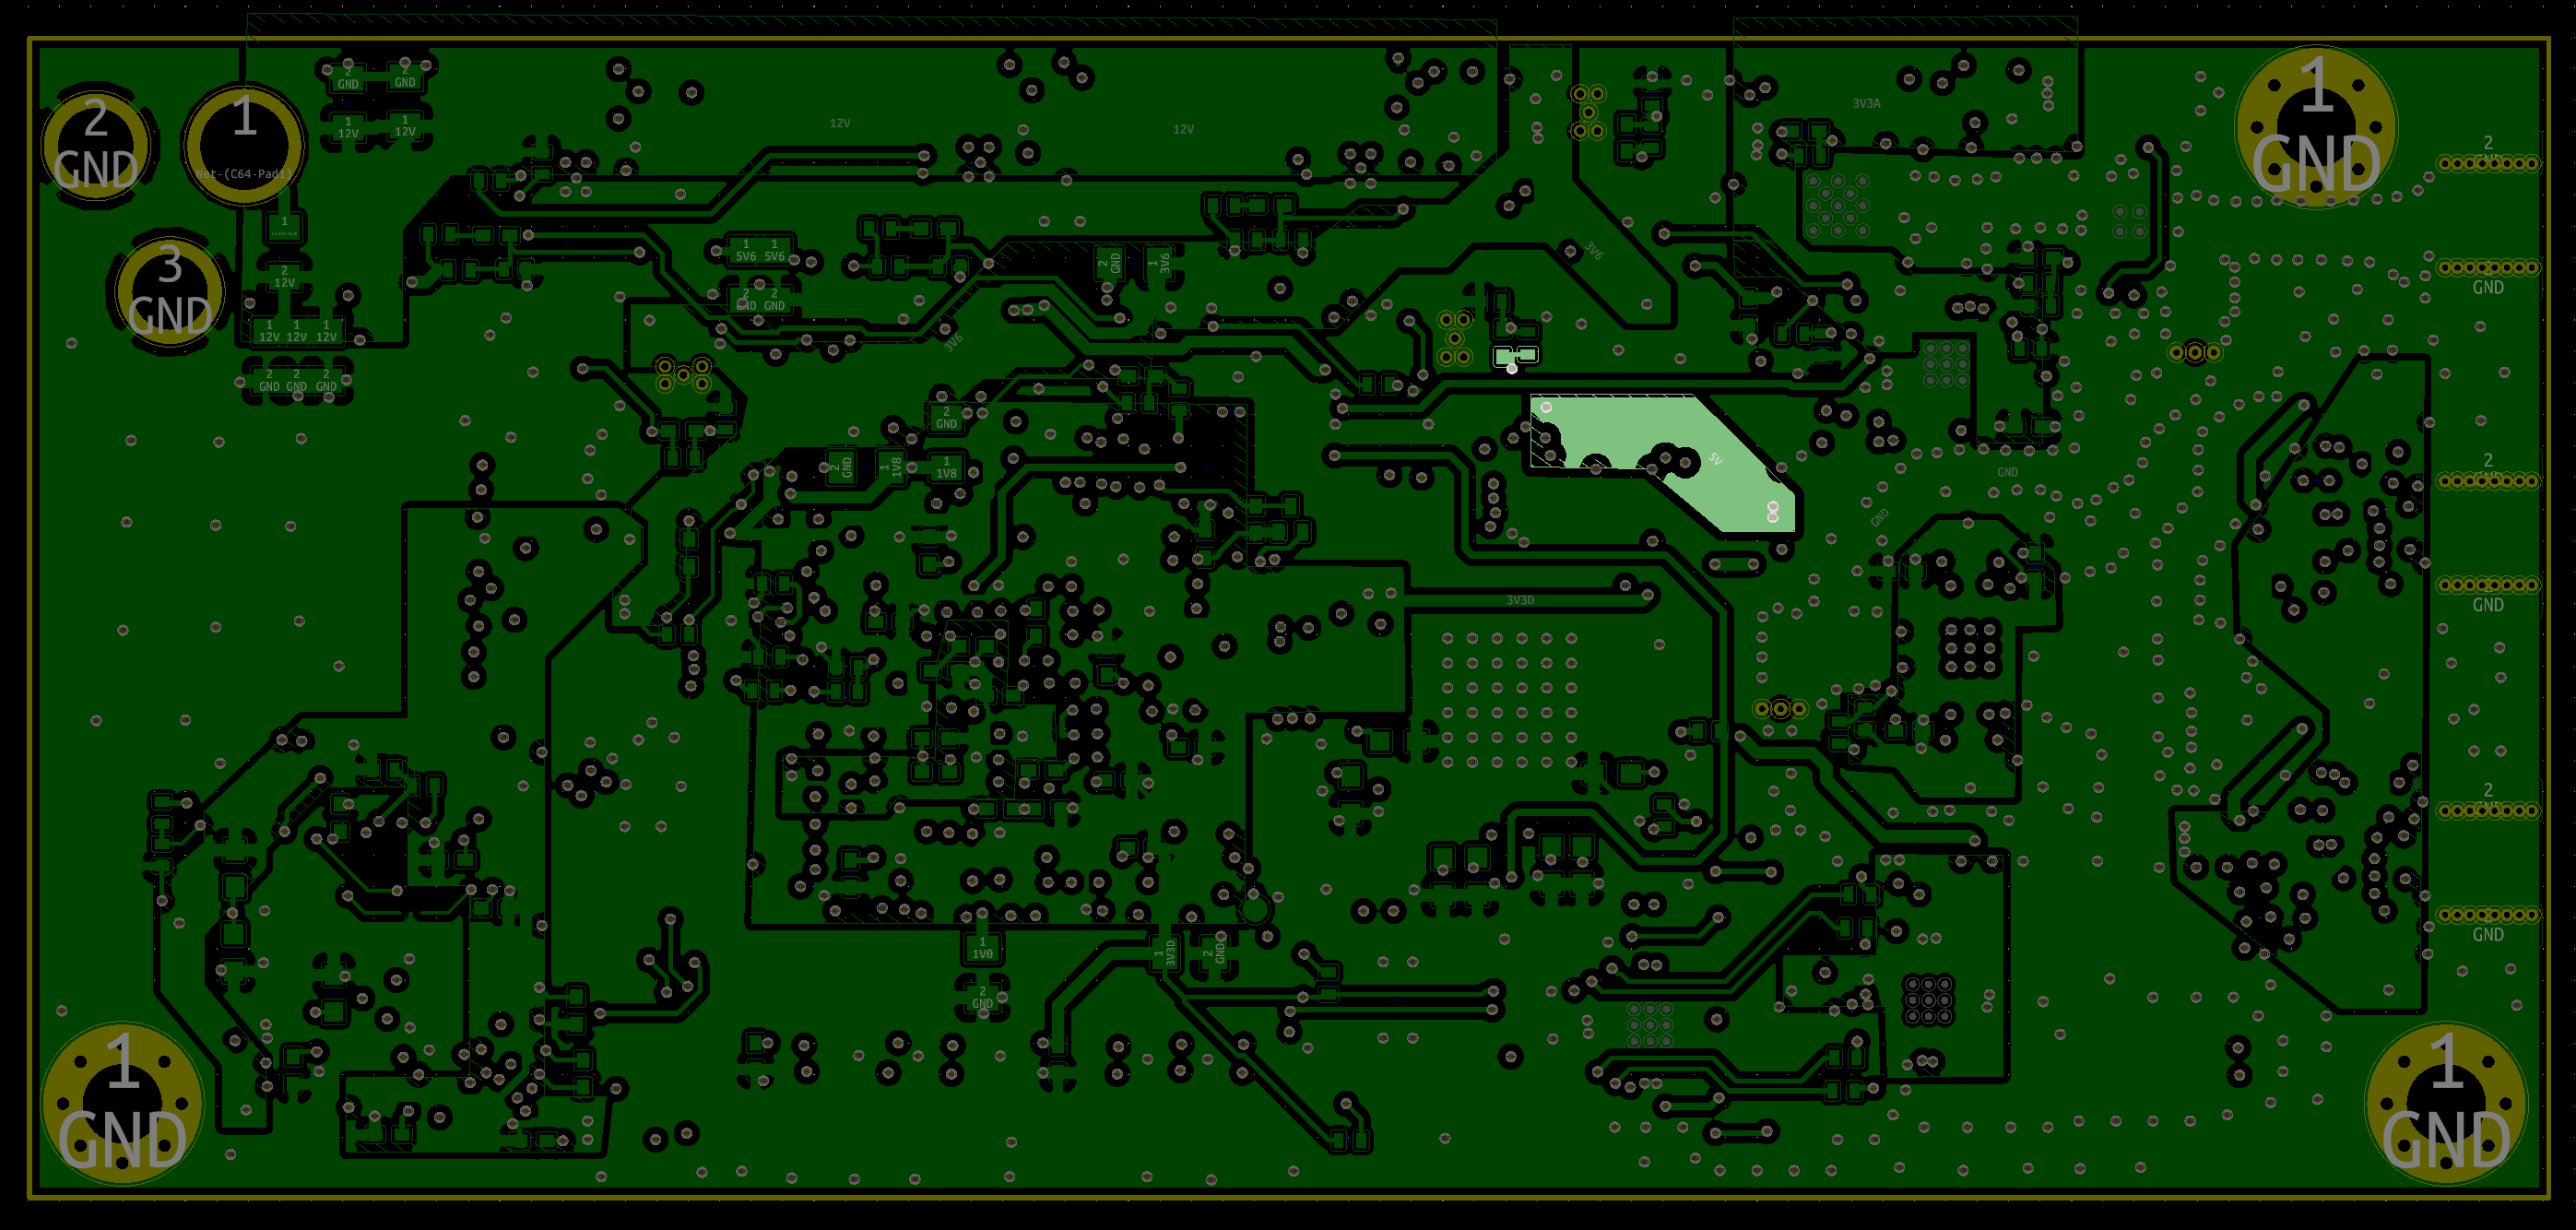
\includegraphics[width=\textwidth]{data/fmcw-layer4-5v.png}
        \caption{A 5V power plane powers one of the inputs to the frequency synthesizer for
          transmission.}
        \label{fig:fmcw-layer4-5v}
\end{figure}

\begin{figure}[h]
        \centering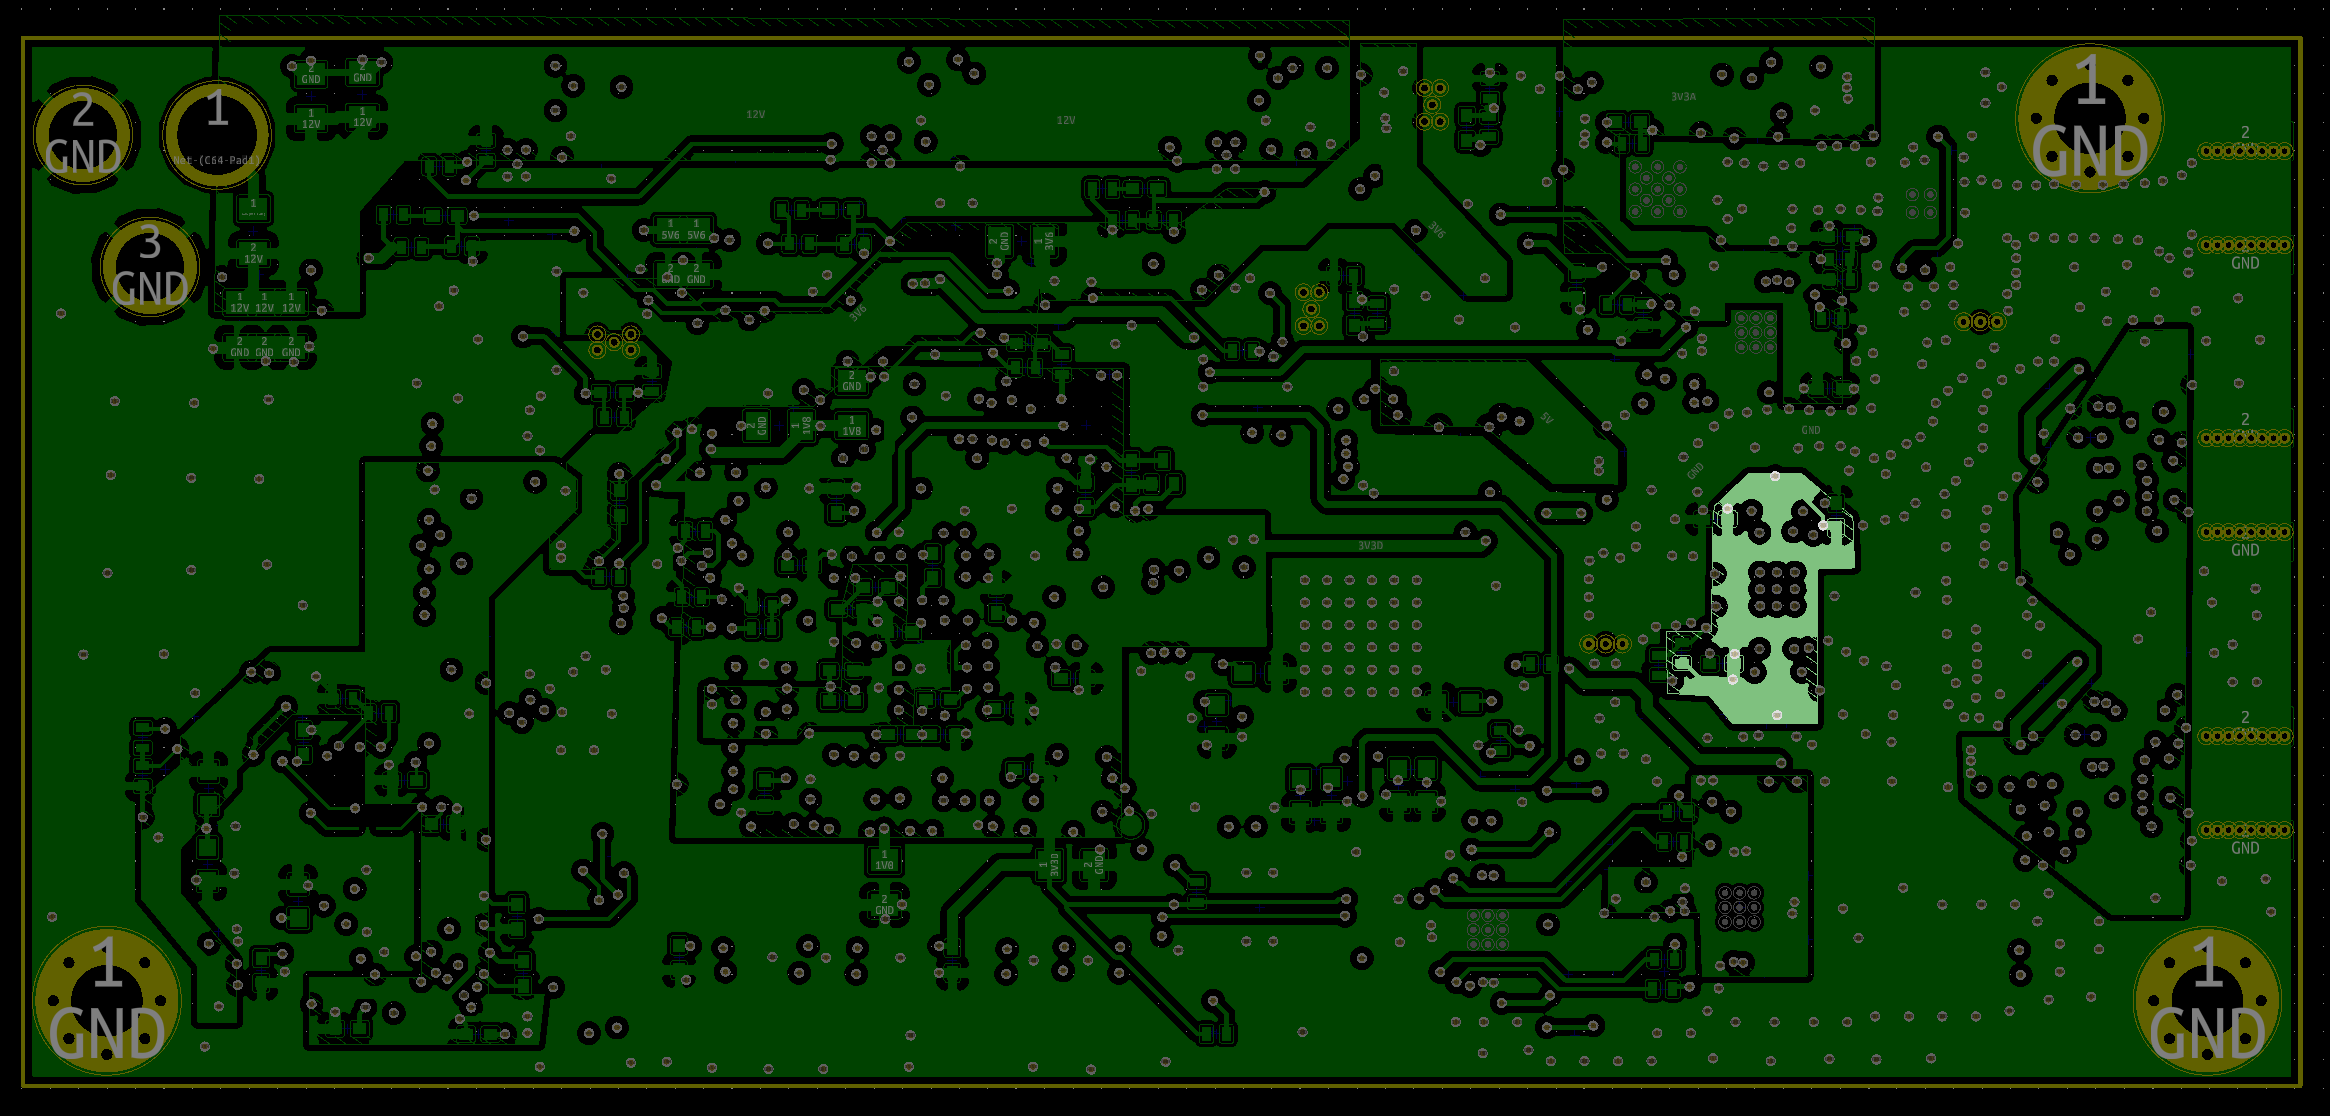
\includegraphics[width=\textwidth]{data/fmcw-layer4-5vf.png}
        \caption{Another 5V power plane is used for to power devices after going through a ferrite
          bead.}
        \label{fig:fmcw-layer4-5vf}
\end{figure}

\section{Board Layout}
\label{sec:board-layout}

There should be a section here on board layout. I.e.\ signal plane, ground plane, power plane,
etc. See High Speed Digital Design for recommendations. Also calculate the capacitance between the
power and ground plane. Btw, this is a great way to further filter noise from the power supplies.

\fixme{I'm not exactly sure where it should go, but there should be a section that documents the use
  of vias, especially for high speed signals. Use page 258 of High Speed Logic to calculate the step
  response, and present the results here. Additionally, mention via best practices such as placing an
  adjacent ground via to any signal via to provide a current return path. Also, the use a multiple
  small vias instead of one large one to minimize inductance. While we're at it, it's probably also
  good to calculate trace inductance for certain important signals. I'm not sure where the equation
  for this is, but it should be in High Speed Design.}

\section{RF Impedance Matching}
\label{sec:impedance-matching}

Document \href{https://en.wikipedia.org/wiki/Via_fence}{via fencing} used. Note the general rule
that spacing between vias should not be more than the RF wavelength divided by 20. I believe the
wavelength is 5cm, but check this and then put this in the documentation. For the impedance line
width I've decided to go with the original design's 14.96mil. I'm a little skeptical of the Mantaro
tool below which seems to not calculate effective impedance. Saturn PCB should be pretty good, and
if you can get OpenEMS to do this that would be the best.

Also document the RF via. Note the parallel ground trace running below it (and the ground plane
above it).

\fixme{I don't think the text below is correct.}.

I'm keeping it for the value of knowing the trace widths used by the original design. However, the
idea that the trace widths are unimportant seems dubious. The PCB calculator built into KiCad should
be used for this. Additionally, it is probably worth looking at the following guides:
\href{https://www.maximintegrated.com/en/app-notes/index.mvp/id/5100#}{Maxim: General Layout
  Guidelines for RF and Mixed-Signal PCBs},
\href{https://hackaday.com/2016/03/23/michael-ossmann-makes-you-an-rf-design-hero/}{Hackaday:
  Michael Ossmann makes you an RF design hero},
\href{https://www.analog.com/media/en/training-seminars/design-handbooks/Basic-Linear-Design/Chapter12.pdf}{Analog}. I
would also look at \href{https://github.com/erichVK5/WilkinsonPowerDividerFootprintGenerator}{this
  tool} for creating a Wilkinson power divider. Also, the trace width for $50\si{\Omega}$ resistors
seems to have been more like 15mil.

Use \href{http://www.mantaro.com/resources/impedance-calculator.htm}{this Mantaro impedance
  calculator} to calculate trace widths. The proper width should be 11.98mil.

The right side of the board houses the RF circuitry (i.e.\ transmitter, receivers and SMA
connectors). The signals are carried to the antennas (a patch-fed horn for transmission and a patch
array for reception) via a $50\si{\Omega}$ coaxial cable. All RF inputs and outputs for components
should match this $50\si{\Omega}$ impedance. The original layout does not seem overly concerned with
the microstrip transmission line width between RF components. They are kept short and generally have
a trace width of about 0.3mm. However, many of them are not even remotely straight and this doesn't
seem to be an issue. Where possible the microstrips should be kept short, straight and with an
unbroken ground plane beneath them. That seems to be all that is necessary for impedance
matching. The patch antennas however will need to be appropriately hooked up in order to match the
$50\si{\Omega}$ impedance. This should be a relatively straightforward calculation. The setup Henrik
uses seems to be the most logical one. He uses a single patch-fed horn antenna for transmission and
a patch array for reception. The horn antenna is made of thin copper. More sophisticated horn
antennas require the ability to weld and probably modeling software (e.g. CST).

%%% Local Variables:
%%% mode: latex
%%% TeX-master: "fmcw-radar"
%%% End:
